% Searchable, impossible-to-miss placeholder macro
\providecommand{\TODO}[1]{\textcolor{red}{\textbf{[TODO: #1]}}}

\chapter{Building \sysname{}} \label{ch:proposition}

This chapter finally presents \sysname{}, the system developed to answer
questions about the 2024 Portuguese manifestos. It becomes evident, throughout this
chapter, that the quality of an answer depends less on the language model used to write it than on the steps that come before.
By the time the model starts writing, the decisions that matter most have already been made, namely
which passages it reads, whether every party is among them, and whether each claim can be traced back to its source.

The catch is that these steps can fail without anyone noticing. A model given
the wrong passages still writes a fluent answer with cited claims. Two of the
failures in this chapter did exactly that, raising no error and going
unnoticed for months (Sections~\ref{subsec:chunking}
and~\ref{subsec:search}). And several techniques that looked promising on
paper were measured and switched off.

%% Running example: q-33 from the dev run current-20261015T050000 (before the
%% code freeze, same retrieval settings). Answer quoted verbatim, cut only.
Before going into how it works, it helps to see how \sysname{} answers a question. To
make each step easier to follow, a question from the evaluation set is used to
trace the system for the entire chapter. The gold question q-33 asks ``O que
propõem os partidos para o salário mínimo?''\footnote{What do the parties
propose for the minimum wage?} It names no party, so it concerns all eight,
and its answer gives each party its own paragraph, every claim traceable to
its manifesto. The following is part of the answer \sysname{} gave to this
question during the development phase.\footnote{In English, ``Aliança
Democrática. The party proposes raising the national minimum wage to 1,000
euros in 2028 [1]. The aim is to ensure that the increase follows inflation
plus productivity gains [2][5]. [\ldots] Iniciativa Liberal. The programme does
not propose a specific value for the minimum wage, but argues for changing
the law to transpose European Directive 2022/2041, setting indicators
[\ldots] that determine the limits of the national minimum wage [13].
[\ldots] Partido Socialista. The party proposes setting, through social
dialogue, a multi-year path of minimum-wage increases that reaches at least
1,000 euros in 2028 [30].''}

\begin{quote}
\small
\textbf{Aliança Democrática.} O partido propõe aumentar o salário mínimo
nacional para 1.000 euros em 2028 [1]. O objetivo é garantir que o aumento
seja feito em linha com a inflação acrescida dos ganhos de produtividade
[2][5]. [\ldots]

\textbf{Iniciativa Liberal.} O programa não apresenta uma proposta de valor
específico para o salário mínimo, mas defende a alteração da legislação para
transpor a Diretiva Europeia n.º 2022/2041, estabelecendo indicadores [\ldots]
que determinem os limites do salário mínimo nacional [13]. [\ldots]

\textbf{Partido Socialista.} O partido propõe estabelecer, através de diálogo
social, uma trajetória plurianual de aumento do salário mínimo que permita
atingir pelo menos 1.000 euros em 2028 [30].
\end{quote}

Every number in the answer comes from a cited passage. And when a party sets
no figure at all, as with Iniciativa Liberal, the answer says so instead
of quietly leaving it out.

The system's design follows five principles, and each section returns to at least one
of them.
\begin{enumerate}
    \item \textbf{Open models.} Every model and library is open source or has
    open weights. Proprietary models appear only in the evaluation phase, for
    the sake of comparison (Section~\ref{subsec:variants}).
    \item \textbf{Strict ahead of time, forgiving at question time.} Work done ahead of time
    can afford to be strict, because nobody is waiting for it. When a call
    fails during indexing, the run stops and later resumes where it stopped, so
    nothing half-finished is ever stored (Section~\ref{subsec:classification}).
    Work done at question time has a user waiting, so it never stops. When a
    call fails there, the step falls back to a simpler version of itself, such
    as spotting party names instead of analysing the question, and the user
    still gets an answer (Section~\ref{subsec:queryanalysis}).
    \item \textbf{Every technique is a switch.} Every technique beyond plain
    search can be turned off on its own, so its contribution can be measured
    on its own (Section~\ref{subsec:variants}).
    \item \textbf{No party is left behind.} Every party in the question's scope
    gets the same number of places in the search and keeps at least one in the answer
    (Sections~\ref{subsec:routing} and~\ref{subsec:context}).
    \item \textbf{Manifestos are the source of truth.} An answer can only come from the
    manifestos, and every claim must point to the passage it came from
    (Section~\ref{subsec:grounding}).
\end{enumerate}

\sysname{} has four parts (Figure~\ref{fig:system-overview}), and each gets a
section of its own.
\begin{itemize}
    \item \textbf{Indexing} (Section~\ref{sec:indexing}) turns the manifestos
    into chunks and embeds them in a database ready to be searched.
    \item \textbf{Retrieval} (Section~\ref{sec:retrieval}) finds the passages
    that answer a question.
    \item \textbf{Generation} (Section~\ref{sec:generation}) writes the answer
    from them.
    \item \textbf{Evaluation} (Section~\ref{sec:evaluation}) measures how well
    each step does its job.
\end{itemize}
Section~\ref{sec:lessons} closes the chapter with what building it taught,
and Appendix~\ref{app:timeline} lists every dated decision in order.

%% Figures in this chapter are rendered from the Mermaid diagrams in
%% docs/architecture.md by scripts/render_diagrams.sh; edit them there.
%% DRAFT (Claude, 2026-10-08): figure captions, to be rewritten.
%% [H] (float package): pinned here so the next paragraph starts after it.
\begin{figure}[H]
    \centering
    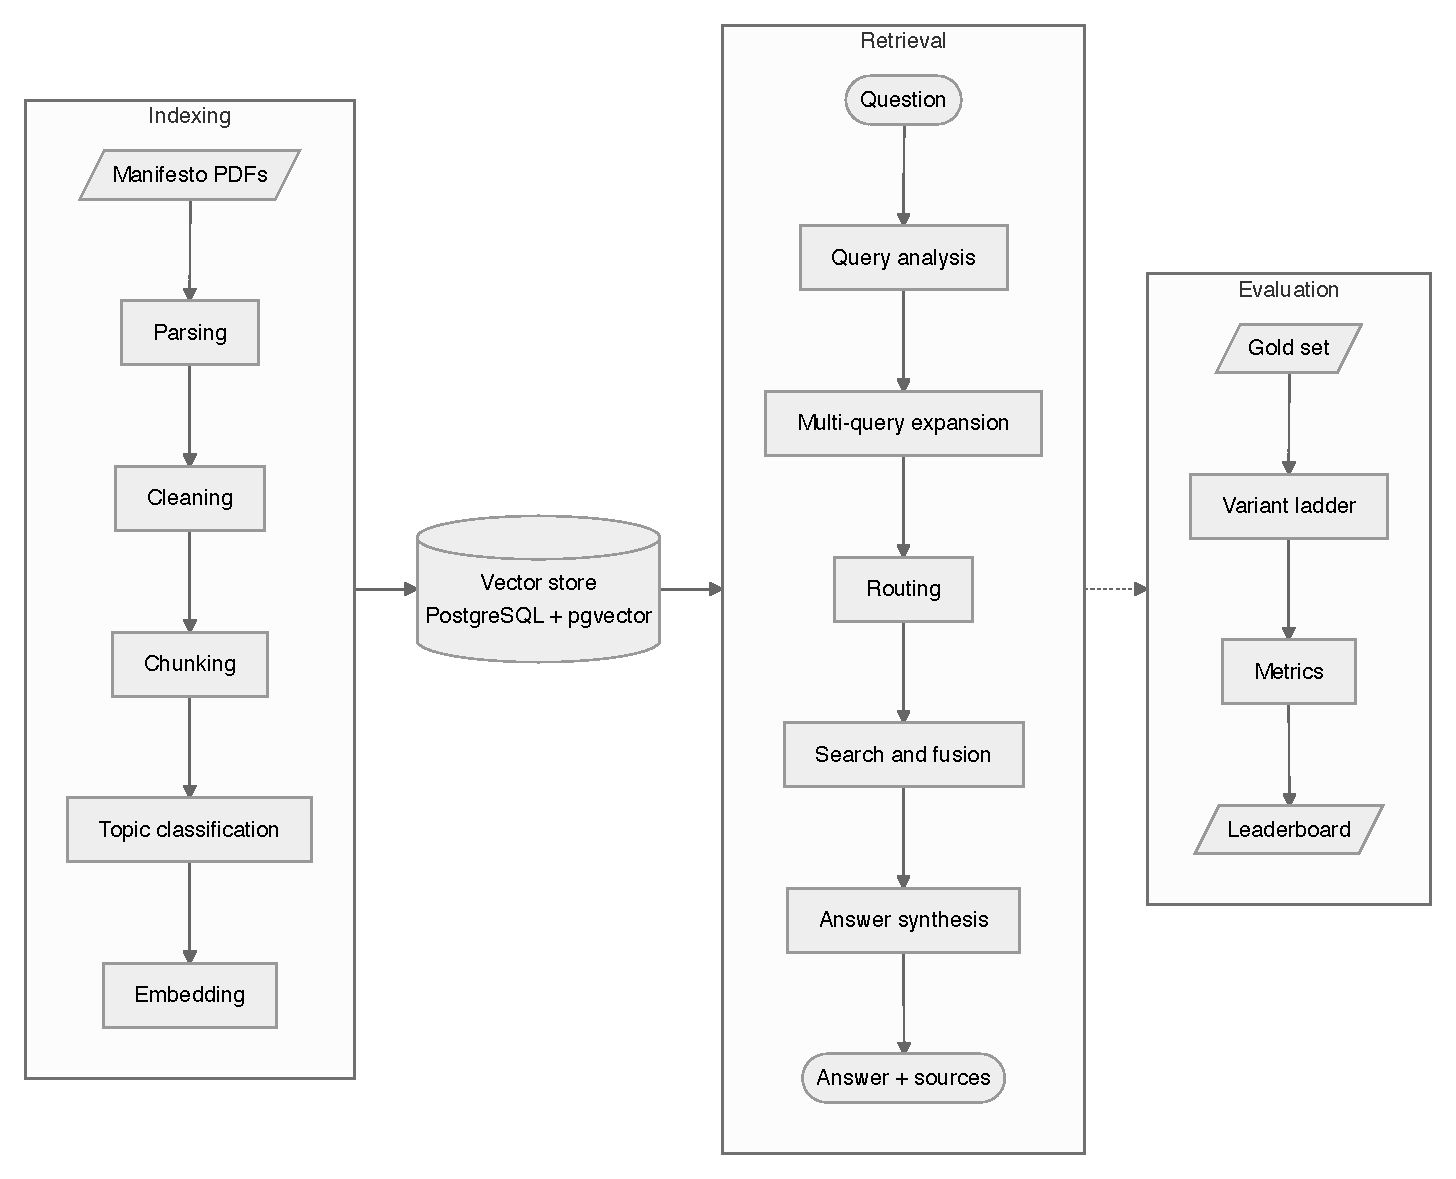
\includegraphics[width=\textwidth]{images/architecture-overview.pdf}
    \caption[Overview of \sysname{}]{Overview of \sysname{}. Indexing builds the vector store that
    retrieval searches for each question, and generation answers from the
    passages retrieved. Evaluation replays retrieval and generation under
    different feature flags. Indexing and evaluation run ahead of time, and
    retrieval and generation run each time a question is asked.}
    \label{fig:system-overview}
\end{figure}

\sysname{} is also cheap enough to try. It can run on a laptop, with the
language model reached through an API. An answer costs about a tenth of a
cent and takes about five seconds on average
(Section~\ref{sec:results-cost}), so a hundred questions cost about ten cents.
The code is public at \url{https://github.com/afonsoni/thesis}, and
Appendix~\ref{app:tooling} explains how to set it up.

\TODO{STYLE: the dated decisions are now in Appendix~\ref{app:timeline}. In the
style pass, drop month-and-year dates from the prose except those that carry
meaning, such as ``a year before it was found''.}

% ============================================================
\section{Indexing} \label{sec:indexing}
% ============================================================

The indexing step prepares the manifestos for search. It runs ahead of time, once for every
change to the corpus, and turns each PDF into short passages, the chunks,
stored in a database with everything retrieval needs to find them. Each
document is parsed into text, cleaned and split into chunks. Each chunk is
then labelled with policy topics, given a short description of where it sits
in its manifesto, encoded as a vector and stored (Figure~\ref{fig:indexing}).
Everything retrieval does later depends on what this stage produces. The
subsections follow the pipeline, except that embeddings come straight after
chunking, because the two share the most instructive failure of this work.

\begin{figure}[htbp]
    \centering
    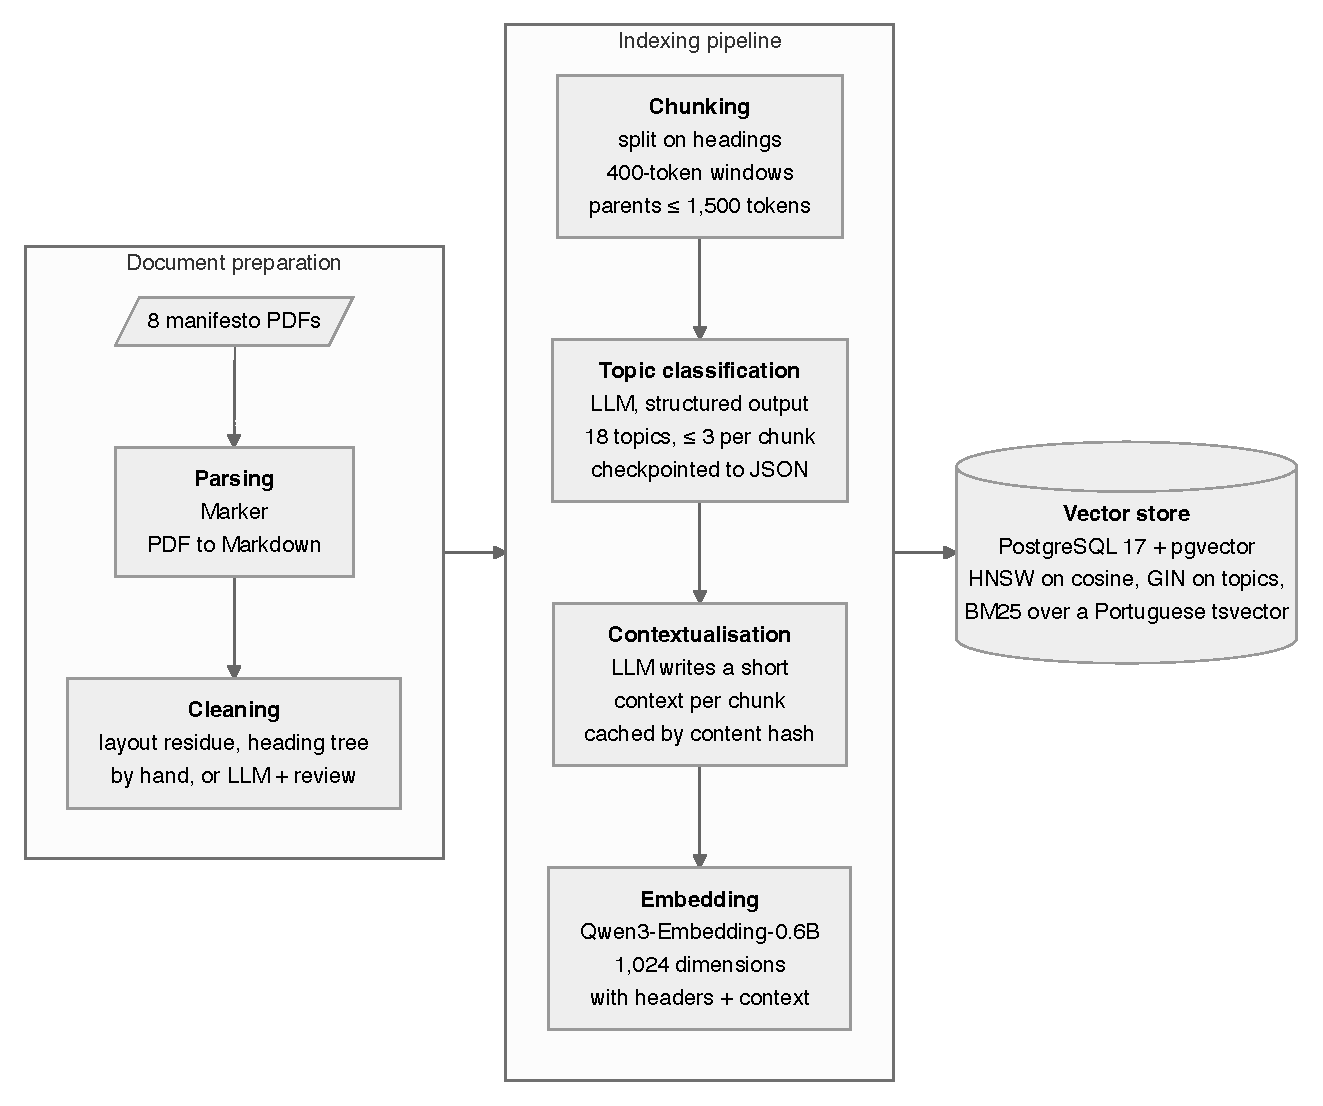
\includegraphics[width=\textwidth]{images/architecture-indexing.pdf}
    \caption[The indexing pipeline]{The indexing pipeline. Document preparation runs once per
    manifesto and its output is reviewed by hand; the indexing pipeline then
    chunks, classifies, contextualises and embeds the cleaned Markdown into the
    vector store.}
    \label{fig:indexing}
\end{figure}

\subsection{Corpus} \label{subsec:corpus}

The corpus is the set of manifestos published for the 2024 Portuguese
legislative election by the eight parties already in the Assembleia da
República, namely Aliança Democrática (AD), Partido Socialista (PS), CHEGA,
Iniciativa Liberal (IL), Bloco de Esquerda (BE), Partido Comunista Português
(PCP), LIVRE and Pessoas--Animais--Natureza (PAN). Two of them ran as
coalitions. The PSD, which sat in the outgoing parliament on its own, stood
with CDS-PP and PPM as AD, and PCP stood with PEV as CDU. In both cases the
document used is the coalition's manifesto. All eight parties were re-elected,
so the corpus also covers the parliament that resulted from the election.

The 2024 election was chosen because it was under way when this work began,
and keeping to parties already in parliament kept the manual preparation
manageable. The price is that the parties voters know least about, those on
the ballot but outside parliament, are left out. The pipeline was later made
easier to extend for this reason (Section~\ref{subsec:cleaning}). Every chunk
also records its election year, so manifestos from other elections could sit
alongside these and support questions about how a position changed over time
(Chapter~\ref{ch:conclusion}).

Table~\ref{tab:corpus} summarises the corpus. The manifestos are long and
uneven, from 94 to 275 pages and from about 31 to 68 thousand words, some
1{,}400 pages and 427 thousand words in all. Each party published its
manifesto as a PDF in February 2024, a few weeks before the vote.
All eight are still published by their parties (Table~\ref{tab:sources}).

\begin{table}[h]
    \centering
    \footnotesize
    \def\UrlBreaks{\do\/\do-\do_}
    \begin{tabular}{|l|p{0.78\textwidth}|}
        \hline
        \textbf{Party} & \textbf{Source (checked October 2026)} \\
        \hline
        AD    & \url{https://ad2024.pt/files/pdf/ad-programa-eleitoral.pdf} \\
        BE    & \url{https://www.bloco.org/media/PROGRAMA_BLOCO_2024.pdf} \\
        CHEGA & \url{https://partidochega.pt/wp-content/uploads/2025/10/Programa_Eleitoral_CHEGA_2024_LQ.pdf} \\
        IL    & \url{https://iniciativaliberal.pt/wp-content/uploads/PROGRAMA_Portugal_com_Futuro_14.pdf} \\
        LIVRE & \url{https://partidolivre.pt/wp-content/uploads/2024/02/Programa_LIVRE_2024_FINAL.pdf} \\
        PAN   & \url{https://www.pan.com.pt/files/uploads/2024/02/Programa-Eleitoral_Legislativas24_Campanhas_2024_PAN-Nacional-1.pdf} \\
        PCP   & \url{https://www.cdu.pt/assets/docs/programa_eleitoral_pcp_2024.pdf} \\
        PS    & \url{https://ps.pt/wp-content/uploads/2024/02/PS-Portugal_Inteiro_2024-6.pdf} \\
        \hline
    \end{tabular}
    \caption[Manifesto sources]{All eight parties still publish their 2024 manifestos at these addresses.}
    \label{tab:sources}
\end{table}

\begin{table}[h]
    \centering
    \begin{tabular}{|l|r|r|}
        \hline
        \textbf{Party} & \textbf{Pages (PDF)} & \textbf{Words (cleaned Markdown)} \\
        \hline
        AD    & 184 & 55{,}474 \\
        BE    & 275 & 66{,}303 \\
        CHEGA & 176 & 53{,}150 \\
        IL    & 166 & 67{,}866 \\
        LIVRE & 155 & 60{,}247 \\
        PAN   & 201 & 30{,}925 \\
        PCP   &  94 & 41{,}070 \\
        PS    & 144 & 51{,}668 \\
        \hline
        \textbf{Total} & \textbf{1{,}395} & \textbf{426{,}703} \\
        \hline
    \end{tabular}
    \caption[The corpus]{Size of each 2024 manifesto, in PDF pages and in words
    after cleaning.}
    \label{tab:corpus}
\end{table}

\subsection{Document parsing} \label{subsec:parsing}

Manifestos are designed for people to read, with multi-column layouts,
decorative covers, running headers, tables of contents and infographics
(Section~\ref{subsec:challenge-documents}). A parser has to recover the
running text in reading order and, ideally, the headings that organise it.

%% Sources: dissertation/HISTORY-GAPS.md §1 (author's answer), commits 80530d7
%% (pdfminer, PyMuPDF) and 1af3074 (Marker).
Four parsers were tried in turn, and only the last one worked well. The first
two were widely used plain-text extractors,
\href{https://github.com/pdfminer/pdfminer.six}{pdfminer.six} and
\href{https://pymupdf.readthedocs.io/en/latest/}{PyMuPDF}, followed by
Microsoft's MarkItDown~\citep{markitdown}. None of them extracted the text
well enough to spare a great deal of repair by hand.
\href{https://docs.llamaindex.ai/en/stable/llama_cloud/llama_parse/}{LlamaParse}
was ruled out without a trial, because it is a paid cloud service.

That last one was Marker~\citep{marker}, and it converted all
eight manifestos. It turns a PDF straight into Markdown, using neural models
for layout detection and optical character recognition (OCR), and it runs
locally. Its
code is under the GPL licence and its model weights under a modified
OpenRAIL-M licence that allows research use, and its optional LLM-assisted
mode was not used. Marker was chosen for clean text, not for its Markdown, but
the Markdown later proved essential. The chunker, written afterwards, splits
each document along its headings (Section~\ref{subsec:chunking}), and it can
only do so because Marker turns the PDF's headings into Markdown ones.

The choice of Marker was pragmatic. Parsing is a means here rather than the object of
study, so no systematic comparison of parsers was run.

\subsection{Cleaning} \label{subsec:cleaning}

Marker's output was usable but not clean. Four of the manifestos, those of AD,
LIVRE, PCP and PS, were corrected by hand, and comparing Marker's output with
the corrected versions shows where the errors were (Table~\ref{tab:cleaning}).

\begin{table}[h]
    \centering
    \begin{tabular}{|l|r|r|r|r|}
        \hline
        \textbf{Party} & \textbf{Words} & \textbf{Headings} & \textbf{Top-level headings} & \textbf{Table lines} \\
        \hline
        AD    & 56{,}817 $\rightarrow$ 55{,}474 & 238 $\rightarrow$ 218 &  3 $\rightarrow$ 2 & 251 $\rightarrow$ 117 \\
        LIVRE & 61{,}491 $\rightarrow$ 60{,}247 & 159 $\rightarrow$ 60  & 57 $\rightarrow$ 1 &  22 $\rightarrow$ 0 \\
        PCP   & 42{,}856 $\rightarrow$ 41{,}070 & 301 $\rightarrow$ 224 & 11 $\rightarrow$ 1 & 118 $\rightarrow$ 9 \\
        PS    & 52{,}307 $\rightarrow$ 51{,}668 & 163 $\rightarrow$ 138 &  1 $\rightarrow$ 1 &  24 $\rightarrow$ 24 \\
        \hline
    \end{tabular}
    \caption{Marker output versus the hand-corrected Markdown.}
    \label{tab:cleaning}
\end{table}

Most of the work went into the heading hierarchy. Marker often promoted
running page headers and section titles to top-level headings, and the LIVRE
manifesto came out with 57 of them, nearly one per page. Each document was
restored to a single title with a consistent tree of sections beneath it.
Tables of contents went next. Marker turns each one into a table full of
section names, and such a table shares words with almost any question while
containing no proposal at all, so it would be retrieved often and answer
nothing. Finally, layout residue such as image links, page anchors, repeated
headers and broken cover titles were removed. Proposal text was left alone.
Between 1.2 and 4.2\% of the words were removed, almost all of them from tables
of contents and page furniture.

%% Source: dissertation/HISTORY-GAPS.md §2 (author's answer, corrected
%% 2026-10-26 to about an hour per manifesto).
Correcting a manifesto by hand took about an hour, often more. That is hardly
acceptable, and even less so once the corpus grows to manifestos from earlier
or later elections, or from parties without a seat in parliament. An automated
cleaner was considered since the beginning, but only after four manifestos were
cleaned by hand did that sort of cleaner become indispensable.
The work was tedious and slow enough to stall the project for a while, and
automating it was no longer optional. The other four manifestos were cleaned by
an automated cleaner written for the purpose and then reviewed by hand.

The cleaner works in two passes. A fixed set of rules first removes the
residue described above. A language model then sees only the candidate
heading lines, never the body text, and returns a decision for each one, to
keep it as a heading at a given level, turn it into body text, or drop it.
Table~\ref{tab:cleaner-plan} shows these decisions on the opening pages of
the Bloco de Esquerda manifesto. A page header that repeats the introduction's
title is dropped, the numbered sections keep their place in the tree, and the
label and title of a chart, which Marker had promoted to headings, go back to
being plain text.

%% Source: data/2_processed/cleaner-cache/be-2024-plan.json (lines 81-125 of
%% the prepared be-2024.md), checked against data/1_markdown/be/be-2024-clean.md.
\begin{table}[H]
    \centering
    \small
    \begin{tabular}{|l|l|}
        \hline
        \textbf{Heading line from Marker} & \textbf{Decision} \\
        \hline
        \texttt{\#\#\# INTRODUÇÃO} & heading, level 2 \\
        \texttt{\#\#\# INTRODUÇÃO} (repeated on the next page) & drop \\
        \texttt{\# 1 Habitação} & heading, level 2 \\
        \texttt{\#\#\# 1.1 A especulação está a tirar-nos as casas} & heading, level 3 \\
        \texttt{\#\#\# **GRÁFICO 1**} & body text \\
        \texttt{\#\#\# Evolução dos preços da habitação em Portugal} & body text \\
        \hline
    \end{tabular}
    \caption[Heading decisions by the cleaner]{Decisions of the cleaner's
    language model on six heading lines of the Bloco de Esquerda manifesto.}
    \label{tab:cleaner-plan}
\end{table}

The model never writes the cleaned file. The code applies its decisions and
then compares the result with the input word by word. Every word in the
output is counted, and if any word appears more often than it did in the
input, the whole output is rejected. Removing words is allowed, since dropping
a running header removes some, but adding or changing one is not, and even a
light paraphrase would bring in a word the manifesto never used. When the
model suggests a tidier version of a heading, the suggestion is kept only if
it passes the same test. Every word in a cleaned file therefore comes from the
manifesto itself. The model was right about most headings but not all, so each
cleaned file was still reviewed by hand.

Run without that review on the four manifestos cleaned
by hand, the cleaner keeps at least 98.4\% of the words the manual cleaning
kept, and at most 2.8\% of its own words are ones the manual cleaning removed.
The headings did not do as well. Section titles match the manual files closely
for AD and PS (F1 of 0.95 and 0.94) but poorly for LIVRE and PCP (0.30 and
0.28), partly because the manual cleaning flattened LIVRE to 60 headings where
the cleaner kept 101. For retrieval the words matter more than the
hierarchy, since the chunker splits on every heading level alike.

\subsection{Chunking} \label{subsec:chunking}

Retrieval works on chunks rather than whole documents, so chunk size sets the
granularity of everything that follows. Small chunks match precisely but lose
their surroundings, while large ones keep context but blur the embedding and
can bury the relevant sentence in the middle (Table~\ref{tab:chunk-sizes}).

\begin{table}[H]
    \centering
    \begin{tabular}{|c|c|}
        \hline
        \textbf{Small chunks} & \textbf{Large chunks}\\
        \hline
        More granular matches & Less granular matches \\
        More diverse sources & Fewer, longer sources \\
        Incomplete context & Relevant text lost in the middle \\
        \hline
    \end{tabular}
    \caption{Trade-offs in chunk size.}
    \label{tab:chunk-sizes}
\end{table}

%% Path example: data/1_markdown/ad/ad-2024-manual.md, headings at lines 1,
%% 565, 567 and 624. Sizes: config.yaml (max_chunk_tokens, chunk_overlap_tokens,
%% max_parent_tokens).
The final design rests on three ideas.

The first is to split each manifesto along its own headings. Every chunk then
belongs to exactly one section and never mixes the end of one topic with the
start of the next. It also carries that section's path, such as
\textit{Programa Social e de Governação da Aliança Democrática $>$ Com
Sensibilidade Social $>$ Saúde $>$ 3.~Medidas} in the AD manifesto.

The second is to cap every chunk at 400 tokens, counted with the encoder's
own tokenizer, so that no chunk is longer than what the encoder reads. A
section that fits stays whole. A longer one is cut into overlapping
\emph{windows}, at paragraph breaks where possible, then at sentence breaks,
and only as a last resort between words. Each window repeats the last 80
tokens of the one before, so a sentence cut at the edge of one window appears
whole in the next. This gives, as an example, 383 chunks for the AD manifesto
and 2{,}815 for the entire corpus.

The third, called small-to-big retrieval, separates the text that is
searched from the text that is read. Search works best on small pieces,
because a short window is about one thing and its embedding matches a
question about that thing closely. Answering works best with more text,
because a proposal often only makes sense next to the sentences around it. So
each small window is embedded and matched on its own, but once it is
retrieved, the generator receives its \emph{parent} instead, that is, the whole section
the window came from. A section can be very long, so a parent is capped at
1{,}500 tokens. A window from a longer section receives the stretch of that
section around it, up to the same cap.

%% Sources: chunk_markdown_file on data/1_markdown (small_to_big, 400/80, parent
%% cap 1500, Qwen3 tokenizer), matched to the q-33 gold keys sha1:ae701d2c (BE)
%% and sha1:9edcbce2 (LIVRE). BE section 819 tokens, 3 windows, child 349 tokens.
%% LIVRE section 5,341 tokens, 16 windows, child 241, parent = windows 0-3,
%% 1,369 tokens.
The minimum-wage question shows both cases. In the Bloco de Esquerda
manifesto, the list \textit{As propostas do Bloco} under \textit{3.1 Salários}
is 819 tokens long and is cut into three windows. The first, of 349 tokens,
opens with the proposal to raise the minimum wage to 900 euros in 2024, and
that window is what the search matches. The generator then reads all 819
tokens of the section, so the answer can also draw on the wage proposals
listed after it. The LIVRE manifesto puts its whole programme for work,
income and social protection in a single section of 5{,}341 tokens, sixteen
windows long, and its first window holds the pledge of a minimum wage of
1{,}150 euros by 2028. Handing the generator all sixteen windows would spend
a large share of the prompt on one party, so it receives the first four
instead, 1{,}369 tokens in all. Figure~\ref{fig:small-to-big} draws both
cases.

\begin{figure}[htbp]
    \centering
    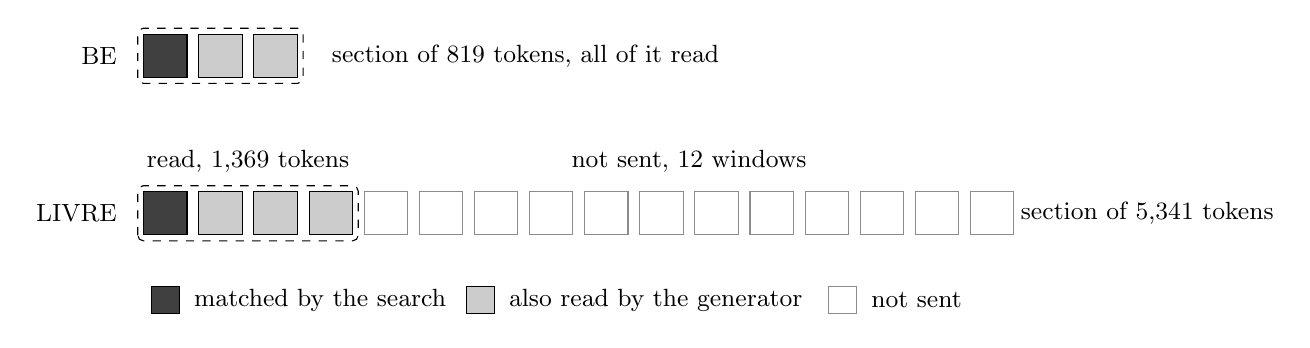
\begin{tikzpicture}[
        win/.style={draw, minimum width=5.5mm, minimum height=5.5mm, inner sep=0pt},
        hit/.style={win, fill=black!75},
        read/.style={win, fill=black!20},
        unsent/.style={win, draw=black!45, fill=white},
        frame/.style={draw, dashed, rounded corners=2pt}]
        \small
        % Bloco de Esquerda: section of 819 tokens, three windows, all read.
        \node[anchor=east] at (-0.5,2) {BE};
        \node[hit]  at (0,2)   {};
        \node[read] at (0.7,2) {};
        \node[read] at (1.4,2) {};
        \draw[frame] (-0.35,1.65) rectangle (1.75,2.35);
        \node[anchor=west] at (2.0,2) {section of 819 tokens, all of it read};
        % LIVRE: section of 5,341 tokens, sixteen windows, first four read.
        \node[anchor=east] at (-0.5,0) {LIVRE};
        \node[hit] at (0,0) {};
        \foreach \i in {1,2,3} {\node[read] at (0.7*\i,0) {};}
        \foreach \i in {4,...,15} {\node[unsent] at (0.7*\i,0) {};}
        \draw[frame] (-0.35,-0.35) rectangle (2.45,0.35);
        \node[anchor=south] at (1.05,0.4) {read, 1{,}369 tokens};
        \node[anchor=south] at (6.65,0.4) {not sent, 12 windows};
        \node[anchor=west] at (10.75,0) {section of 5{,}341 tokens};
        % Legend.
        \node[hit, minimum width=3.5mm, minimum height=3.5mm] at (0,-1.1) {};
        \node[anchor=west] at (0.25,-1.1) {matched by the search};
        \node[read, minimum width=3.5mm, minimum height=3.5mm] at (4.0,-1.1) {};
        \node[anchor=west] at (4.25,-1.1) {also read by the generator};
        \node[unsent, minimum width=3.5mm, minimum height=3.5mm] at (8.6,-1.1) {};
        \node[anchor=west] at (8.85,-1.1) {not sent};
    \end{tikzpicture}
    \caption[Small-to-big retrieval]{Small-to-big retrieval on two gold
    passages for the minimum-wage question. Each square is one window of up to
    400 tokens, and the overlap between windows is not drawn.}
    \label{fig:small-to-big}
\end{figure}

\paragraph{How the design was reached.} The current design is the fourth
attempt. The three attempts before this one measured chunks in words or characters, the
units of the common splitting libraries, while the encoder measures what it
reads in tokens. Nothing in between compares the two.

The first prototype cut chunks of 1{,}000 words, which was the splitter's default.
Meanwhile, the encoder, \texttt{all-MiniLM-L6-v2}, read at most 256 tokens. Later
versions moved to 1{,}000 and then 1{,}600 characters, in line with the common advice
of the time, which favoured larger chunks as models grew to read longer
inputs (Section~\ref{subsec:sota-indexing}).

The mismatch came to light once chunk lengths were measured in tokens, the
unit the encoder actually reads. The encoder then in use, Serafim
(Section~\ref{subsec:embeddings}), which read at most 128 tokens, dropped the rest
without any warning. At 1{,}600 characters the median chunk was 365 tokens
long, so 89.5\% of the chunks were cut short and only 37.3\% of the corpus text
reached the embeddings. After testing with a simple probe, the effect was confirmed.
Queried with its own opening, a chunk came first, with a cosine similarity of 0.986.
Queried with its own closing lines, it did not reach the top five.

%% Source: chunk_markdown_file on data/1_markdown/ad/ad-2024-manual.md with the
%% char strategy (1,600 / 200), Serafim tokenizer; the phrase "salário mínimo
%% para 1.000€" starts at token 245 of a 470-token chunk (3. Medidas, window 0).
The minimum-wage question shows what that meant in practice. In the AD
manifesto, the pledge to raise the minimum wage to 1{,}000 euros by the end
of the legislature sat at token 245 of a 470-token chunk, far past the 128
that Serafim read. The chunk could still be found through its opening lines
on social benefits, but the pledge itself never reached the embedding. Most
of each chunk was invisible to retrieval, while every component ran without an error, which
is exactly the kind of quiet failure this chapter keeps returning to
(Section~\ref{sec:lessons}).

%% Checked 2026-10-26: the vault note "5 - rag/Chunking.md" (written early, per
%% the author) lists 128 to 2048 and the same three metrics as the LlamaIndex
%% post (Ravi Theja, 5 Oct 2023). LlamaIndex's SentenceSplitter documents
%% chunk_size as "The token chunk size for each chunk". The DataCamp tutorial
%% (Eugenia Anello, 12 Apr 2024) calls the same LlamaIndex setting characters.
The irony is that the right unit had been in the research notes from the
start. Early in the work, the notes planned to compare chunk sizes from 128 to
2{,}048, following a LlamaIndex tutorial~\citep{theja2023chunksize}. In
LlamaIndex, those sizes are counted in tokens.

In short, one number had to respect two different limits. The first is how
much the encoder can read, the \emph{retrieval limit}, and text past it is
dropped without warning. The second is how much the language model can read,
the \emph{generation limit}, which chunks of this size never come close to.
The chunks had been sized with the second limit in mind, but they were handed
to the encoder, which is bound by the first. Two changes fixed this. Chunk
length is now counted with the encoder's own tokenizer, so no window is longer
than what the encoder reads. And small-to-big retrieval gives each limit its
own text, a small window for the encoder and the whole section for the
language model. No chunk has been truncated since, and the old
character-sized chunks are kept only as a baseline to compare against.

\subsection{Embeddings} \label{subsec:embeddings}

The encoder decides which chunks a question can find. For this corpus it has
three requirements. It has to handle European Portuguese. It has to be trained
for \emph{retrieval}, which means placing a short question close to the longer
passage that answers it, a different task from judging whether two sentences
mean the same thing. And it has to read a whole chunk at once.

\paragraph{Language.} Before choosing a model, there was a more basic choice
to make, whether to work in Portuguese at all. Early on, Portuguese models were
scarce enough that translating the whole corpus into English, where stronger
models existed, looked like a way around the problem. The idea was dropped for
three reasons. In political text the exact wording matters. A translation
would put a layer of interpretation between the voter and the party. And
studying RAG in European Portuguese was, and still is, part of what this work
set out to do.

%% Sources: dissertation/HISTORY-GAPS.md §3 (pre-thesis shortlist, author's
%% answer). Only three encoders were ever committed (git history):
%% all-MiniLM-L6-v2, Serafim, Qwen3-Embedding-0.6B. The author tried a couple
%% of other encoders locally after MiniLM, without committing them (author,
%% 2026-10-27). The pre-thesis also names
%% Gemini 2.0 Flash, so it postdates Dec 2024 and predates Qwen3-Embedding
%% (June 2025).
\paragraph{Candidates.} Before any code was written, the preliminary research
used MTEB~\citep{mtebmassivetextembedding} to shortlist encoders that support
Portuguese, namely BERTimbau~\citep{souza2020bertimbau},
Sentence-BERT~\citep{reimers2019sentencebert},
\texttt{paraphrase-multilingual-MiniLM-L12-v2} and
\texttt{multilingual-e5-large-instruct}~\citep{wang2024multilinguale5textembeddings},
together with two commercial services, OpenAI's \texttt{text-embedding-3-large}
and Google's \texttt{text-multilingual-embedding-002}. The commercial services
were set aside so that \sysname{} could run on open models alone. A shortlist
drawn up before any code exists can only go so far, and this one was soon
overtaken. Neither encoder that \sysname{} ended up relying on was on it.
Serafim was not included, and Qwen3-Embedding had not yet been released.

\paragraph{First choices.} The first prototype used \texttt{all-MiniLM-L6-v2},
a small and widely used default encoder, so that the rest of the pipeline
could be built and tested before the choice of model mattered. It reads
English only, so its answers were poor, as expected, but it showed that the
pipeline worked end to end. With that in place, a couple of the open
candidates were swapped in and judged by the answers they produced. There was
no gold set yet to measure them against, since it came much later. The search
then turned to encoders trained for retrieval in European Portuguese, which
the shortlist did not cover, and one stood out among them,
\texttt{serafim-900m-portuguese-pt-sentence-encoder-ir}, from the Serafim
family of European Portuguese encoders~\citep{gomes2024serafim}. Serafim
looked right on every visible criterion. It was trained on European
Portuguese, came in a variant built for retrieval and was recent. Its authors
reported it as the state of the art for Portuguese, and on their Portuguese
retrieval test the retrieval variant beat every model they
compared~\citep{gomes2024serafim}. That comparison left out the strongest
multilingual encoders, though, and used a machine-translated test set.
%% Checked 2026-10-26: Table 4 of arXiv 2407.19527, MRR@10 0.854 for Serafim
%% 900 IR against 0.741 for the best non-Serafim model (GTE); test set is MS
%% MARCO (TREC DL 2019) translated with Google Translate.
It was the first encoder with which
\sysname{}'s answers became acceptable.

%% Checked 2026-10-26: the model's sentence_bert_config.json sets max_seq_length
%% 128, its DeBERTa-v2 config allows 512 positions, and the paper (arXiv
%% 2407.19527) builds the 900M model on Albertina PT-PT and tunes the IR variant
%% on mMARCO. The paper states no sequence length.
\paragraph{Reversal.} One property of Serafim was never checked when it was
chosen, the length of text it reads. It ships set to read at most 128 tokens and silently discards the rest, which
caused the truncation described above. The cap could have been raised, since
the network underneath, Albertina, accepts 512 tokens. But the retrieval
variant was tuned on mMARCO, a translation of MS~MARCO whose passages run to a
few sentences~\citep{gomes2024serafim}. There is no evidence that it would
represent well a passage as long as the median chunk of the time, 365 tokens
(Section~\ref{subsec:chunking}), and 512 tokens would still have bound the size
of every chunk. It was replaced by
\texttt{Qwen3-Embedding-0.6B}~\citep{zhang2025qwen3embedding}, an encoder
built on a language model and trained for retrieval, which reads up to 32
thousand tokens, so the encoder no longer limits chunk size at all. It is also
smaller than Serafim (0.6 against 0.9 billion parameters) and produces shorter
vectors (1{,}024 against 1{,}536 numbers). It scores 78.9 on retrieval in MTEB-PT, a Portuguese
benchmark published after the switch~\citep{okamura2026mtebpt}, which does not
score the Serafim variant used here, so no like-for-like comparison exists.

%% Source: the model's config_sentence_transformers.json (query prompt, empty
%% document prompt) and src/rag/indexing/embedder.py (encode_query).
The new encoder also changed how questions are encoded. A question and the
passage that answers it look different. The question is short and asks, while
the passage is long and states. A \emph{symmetric} encoder treats both texts
the same way, which suits comparing two similar sentences. Qwen3-Embedding,
like most current retrieval encoders, is \emph{asymmetric}. Every question is
prefixed with a short instruction that names the task, \textit{Given a web
search query, retrieve relevant passages that answer the query}, while the
chunks are encoded as they are. The instruction tells the model which side of
the match a text is on. Leaving it out at search time would place questions
in the wrong part of the vector space, and nothing would report the mistake.
\sysname{} therefore encodes questions and chunks through two separate
functions, and only the question path adds the instruction.

The move from a Portuguese model to a multilingual one is a trade-off rather
than a plain upgrade. A model not built around European Portuguese may handle
words whose meaning changes between varieties less well (such as was seen with
\textit{propinas} and \textit{renda} in Section~\ref{subsec:challenge-language}).
%% Sources: commits f896f61 (small-to-big with Serafim, 112-token windows, 0%
%% truncated on AD) and ee2ff51 (switch to Qwen3, 30 minutes later). Prefix
%% length: party | section path + LLM context for all 2,815 chunks, counted
%% with the Serafim tokenizer, median 131, 59% at or above 126.
The design itself does not rule Serafim out. Small-to-big retrieval separates
the window that is embedded from the text the generator reads, so \sysname{}
could run Serafim again by changing its configuration alone, with windows of
about 112 tokens that fit inside its 128. That configuration did run briefly,
right after the truncation was fixed and before the switch, but it was never
compared on the gold set. The obstacle today is contextual retrieval
(Section~\ref{subsec:contextual}). The party, section path and context
written before each chunk take a median of 131 Serafim tokens on their own,
more than its whole window, so for most chunks the encoder would never reach
the chunk's own text. Using Serafim would mean giving up contextual retrieval,
raising its limit towards 512 tokens, a length its retrieval tuning never
covered, or embedding the context separately from the chunk, which changes the
index. Qwen3-Embedding was chosen because it removed the limit altogether, not
because Serafim could not be made to fit.

Whether a long-window Portuguese encoder would do better on this corpus is an
empirical question. Answering it means indexing the corpus once per encoder and
comparing retrieval on the same gold set, which was not done before the code
was frozen for the final evaluation (Chapter~\ref{ch:conclusion}).

\subsection{Contextual retrieval} \label{subsec:contextual}

A chunk cut from the middle of a section is an orphan. It no longer says which
party wrote it or what the section is about, and 58\% of the chunks in this
corpus (1{,}634 of 2{,}815) contain no heading at all. Voters do not help
either, since they rarely use the manifesto's own words.

Contextual retrieval~\citep{anthropic2024contextual} gives each orphan its
bearings. Before embedding, a language model reads the chunk alongside its
section and writes a sentence or two placing it in context. The chunk is then
embedded together with that context and its party and section path, and the
context is added to the keyword index as well. The stored text is left untouched, so citations and
the gold set still point at exactly what the manifesto says. Contexts are
cached by content, so rebuilding the index never pays for them twice, and, as
in every other step of indexing, a context that cannot be written stops the
run.

%% Sources: commit 524d9ea; runs current-20261011T210519/211256 (plain hybrid),
%% contextual-20261011T210746/211528 (paths), contextual_llm-20261011T211023/
%% 211803 (paths + context), top_k 5, averaged over the two passes.
It paid off (Table~\ref{tab:contextual}). The comparison ran on all 61 gold
questions, twice, with the retrieval metrics of Section~\ref{subsec:metrics}.
The section paths alone gave about half of the gain, and the context written
by the language model gave the rest. The gains in recall and nDCG are larger
than the noise between runs, since their 95\% confidence intervals stay above
zero. It has been the default index since.

\begin{table}[H]
    \centering
    \begin{tabular}{|l|c|c|c|}
        \hline
        \textbf{Embedded text} & \textbf{Recall} & \textbf{MRR} & \textbf{nDCG} \\
        \hline
        Chunk only & 0.731 & 0.729 & 0.649 \\
        Party and section path, then chunk & 0.756 & 0.785 & 0.680 \\
        Party, section path and context, then chunk & \textbf{0.777} & \textbf{0.811} & \textbf{0.706} \\
        \hline
    \end{tabular}
    \caption[Contextual retrieval]{Retrieval with and without contextual
    retrieval, averaged over two runs of the 61 gold questions with five
    chunks retrieved per question, the setting of the time. Against the first
    row, the last gains +0.046 in recall (95\% CI +0.011 to +0.089) and +0.057
    in nDCG (+0.025 to +0.095).}
    \label{tab:contextual}
\end{table}

%% q-33 chunk: data/1_markdown/ad/ad-2024-manual.md re-chunked with the
%% production settings (sha1:cfa43c8ce1...), context from
%% data/2_processed/contexts-gemma-4-31b-it.json. Quoted verbatim, cut only.
\paragraph{The running example.} The gold answer to q-33 lies in 20 chunks
spread over 17 sections of the eight manifestos.
Figure~\ref{fig:q33-chunk} shows one of them, the AD's goals for social and
labour policy, as the encoder reads it. The section is short, 266 tokens, so
it fits in a single chunk, and here the chunk the search matches and the
section the generator reads are the same text.

\begin{figure}[htbp]
    \centering
    \fbox{\begin{minipage}{0.93\textwidth}
    \small
    \textbf{Aliança Democrática \textbar{} PROGRAMA SOCIAL E DE GOVERNAÇÃO DA
    ALIANÇA DEMOCRÁTICA $>$ COM SENSIBILIDADE SOCIAL $>$ POLÍTICAS SOCIAIS,
    TRABALHO E SEGURANÇA SOCIAL $>$ 2.~Metas}

    \medskip
    \textit{Metas do programa eleitoral da Aliança Democrática no âmbito das
    políticas sociais e de trabalho, focando-se no aumento do salário mínimo,
    do CSI, combate à precariedade e incentivos à produtividade.}

    \medskip
    2. Metas \\
    \textbullet{} Reduzir a taxa de pobreza entre os trabalhadores; \\
    \textbullet{} Aumentar o valor de referência do Complemento Solidário para
    Idosos (CSI) para um valor de 820 euros em 2028 [\ldots]; \\
    \textbullet{} Aumentar o salário mínimo nacional para 1.000 euros, em
    2028, e aumentar o salário médio para 1.750 euros, em 2030, com base em
    ganhos de produtividade e diálogo social; \\
    {}[\ldots]
    \end{minipage}}
    \caption[A chunk as the encoder reads it]{One of q-33's gold chunks as the
    encoder reads it. The first line is the party and section path, the line in
    italics the context written by the language model, and the rest the
    manifesto text, cut here for space. Only the manifesto text is stored as
    the chunk itself.}
    \label{fig:q33-chunk}
\end{figure}

\subsection{Topic classification} \label{subsec:classification}

Every chunk is also labelled with policy topics, so that a search could be
limited to, say, passages on housing. No labelled data exists for Portuguese
manifestos, and the documents do not tag their own sections consistently, so
the labels are assigned by a language model during indexing. The 18 categories
(Table~\ref{tab:topics} in Appendix~\ref{app:results}) come from reading the
manifestos for recurring policy areas and from two public comparators of party
programmes~\citep{expresso-comparador, politicaativa-comparar}. A chunk can
carry several topics, because a proposal to build student residences concerns
housing, education and youth at once. To classify them, the model reads chunks
in batches of 15 and returns, for each, its categories, a confidence score
and keywords, checked against a schema.

In the end, the labels matter less than planned. A search limited to one
topic turned out to miss relevant passages that had been labelled under
another, so the topic filter is off in the production system
(Section~\ref{subsec:routing}). The labels are now used only by the
evaluation variants that turn the filter back on, to measure what it costs.

Building the classifier still taught two lessons.

%% Source: commit c298e4b (removed TOPIC_KEYWORDS and
%% classify_topics_fallback, which matched keywords as substrings).
\paragraph{A failed call stops the run.} The first version of the classifier
had a backup plan. Whenever a call to the model failed, it labelled the batch
itself by looking for a short list of words per topic, such as
\textit{hospital}, \textit{médico} or \textit{SNS} for health, and
\textit{casa}, \textit{renda} or \textit{arrendamento} for housing. Such
matching is crude. It cannot tell a proposal on hospitals from a passing
mention of one, and since it matched fragments of words, \textit{casa} also
fired inside \textit{casamento}, so a passage on marriage could be labelled as
housing. Under free-tier rate limits, calls failed often, so the backup ran
often too. The run always finished and every chunk got labels, but some came
from the model and some from the word lists, and nothing recorded which. The
backup even filled in the same confidence score, from the number of words it
had matched. A
corpus that looked fully labelled was in fact labelled two different ways.

The backup was removed. A failed call now stops the run, and a checkpoint
saves the labels already obtained, so the next run resumes where the last one
stopped instead of starting over. A stopped run is visible and cheap to
finish, while a silently degraded one is neither. This became the rule for
every step of indexing.

\paragraph{The prompt asked for too many labels.} A check by hand of 30 AD
chunks found the first label right in about 29 of them, but a wrong extra
label on about 8, such as a passage on tourism also tagged as health. The
model, meanwhile, rated its own confidence 4 or 5 out of 5 on every chunk. The
prompt was to blame. It asked for ``MÚLTIPLAS categorias'',\footnote{Multiple categories.} which reads as a request for several, and allowed up to four. It
now asks for the main topic first, and for a further label only when the chunk
makes a concrete proposal in that area, with three at most. The corpus was
labelled again with the new prompt.

\subsection{Vector store} \label{subsec:vectorstore}

The store holds one vector per chunk, with its text and metadata (party,
section path and topics), and answers nearest-neighbour searches filtered by
that metadata.

\paragraph{Candidates and first choice.} The preliminary research surveyed
dedicated vector databases, namely Faiss, Pinecone, Qdrant, Milvus, ChromaDB
and Weaviate, with ANN-Benchmarks~\citep{aumuller2020annbenchmarks} as a
reference, and all but Pinecone are open source. Milvus came first, on its
reputation among practitioners for being light and fast, and because a
dedicated vector database seemed the natural tool for the job. In practice it
only ever ran as Milvus Lite, a single local file, because setting up a Milvus
server proved more trouble than the project warranted.

\paragraph{Reversal.} A few months later the store was replaced by
PostgreSQL~17 with the pgvector extension~\citep{pgvector}, which had not been
on the surveyed list at all. The survey had asked \emph{which vector
database}, and an extension to a general relational database fell outside the
question. Three reasons made the case. A corpus of a few thousand chunks does
not need a separate vector service, PostgreSQL was already a familiar tool
with nothing new to learn, and filtering by metadata becomes plain SQL instead
of a
product-specific language. A fourth benefit was not planned for. PostgreSQL
ships with full-text search for Portuguese, so when hybrid retrieval arrived a
year later (Section~\ref{subsec:search}), its keyword half needed no new
component. The table layout and its indexes are described in
Appendix~\ref{sec:tooling-schema}.

% ============================================================
\clearpage
\section{Retrieval} \label{sec:retrieval}
% ============================================================

Indexing happens once, ahead of time. Retrieval happens every time someone
asks a question. This split between work done ahead of time and work done at
question time is the usual shape of a RAG system, and it explains a principle
met throughout this chapter. Work done ahead of time can be slow and strict. Indexing stops at the first
failed call, because a bad label or a missing context would be stored for good
(Section~\ref{subsec:classification}). Work done at question time must answer
within seconds, and a weaker answer is better than none, so every step at
question time falls back to a
simpler behaviour when a call to the language model fails.

Retrieval turns a question into a ranked set of manifesto passages in five
steps (Figure~\ref{fig:retrieval}). The question is first analysed, to find
which parties and topics it concerns. It is then expanded into several
reformulations, routed to a search strategy and searched, and the ranked lists
that come back are fused into one. Every technique beyond plain dense search
sits behind a switch, a \emph{feature flag}, and can be turned off on its own,
which is what lets the evaluation (Section~\ref{sec:evaluation}) measure what
each one adds. Many of the techniques seen here come from the \textit{RAG from Scratch}
series~\citep{rag-from-scratch}, and the rest come from practitioner tutorials and
blog posts. Again, the minimum-wage question follows each step below.

\begin{figure}[htbp]
    \centering
    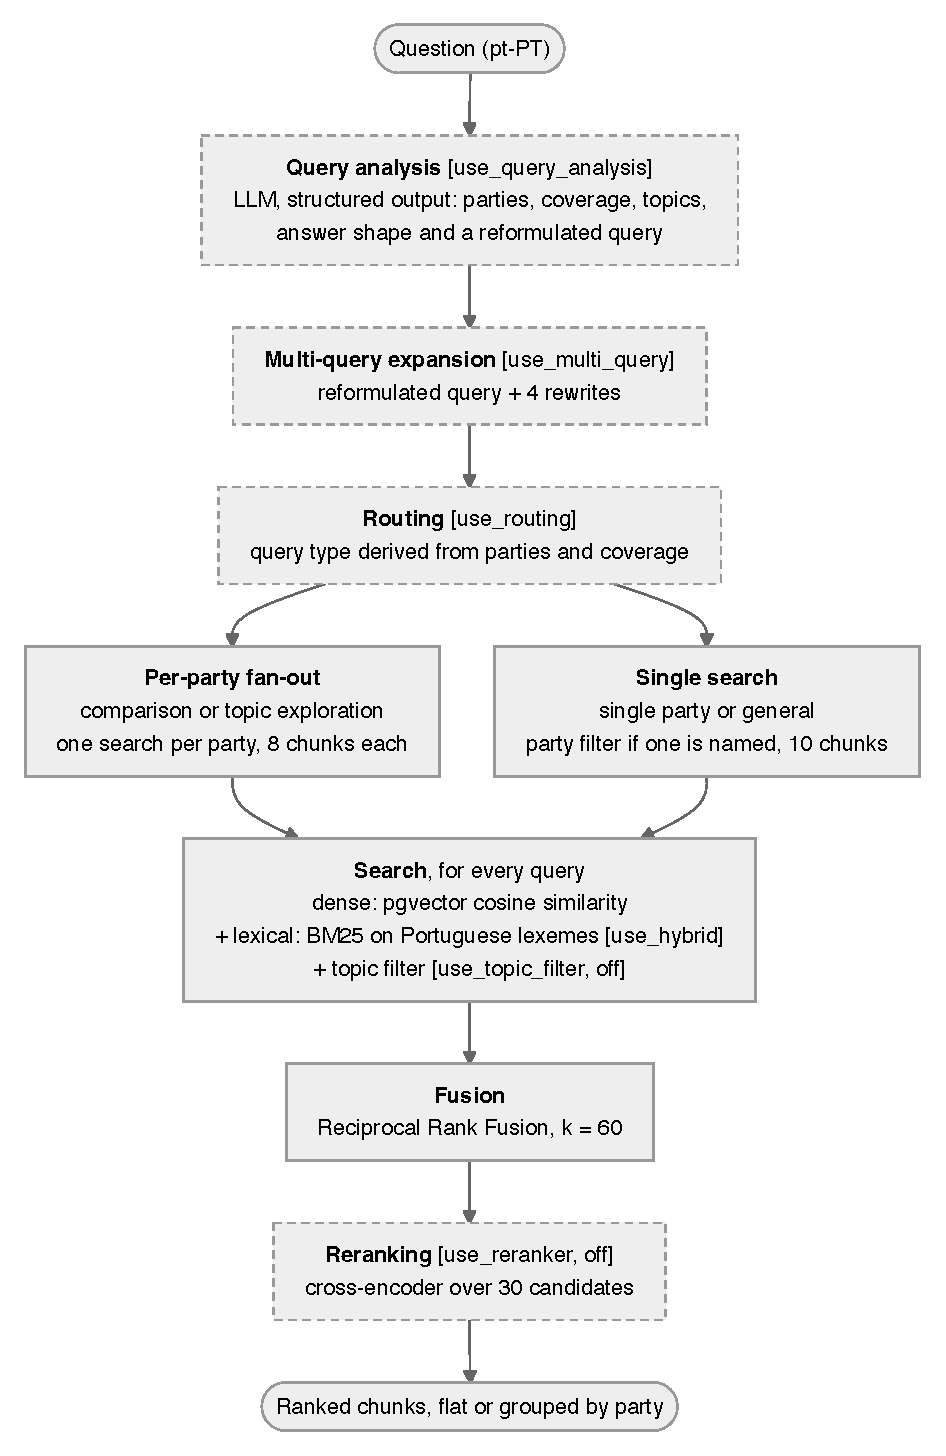
\includegraphics[width=0.85\textwidth]{images/architecture-retrieval.pdf}
    \caption[The retrieval pipeline]{The retrieval pipeline. Dashed stages are
    switched by the feature flag in brackets, and with the flag off a stage
    falls back to its simplest form (Section~\ref{subsec:variants}). Reranking
    and the topic filter are off by default. A question that names only
    parties outside the corpus skips search. Answer synthesis follows in
    Figure~\ref{fig:generation}.}
    \label{fig:retrieval}
\end{figure}

\subsection{Query analysis} \label{subsec:queryanalysis}

Every chunk in the store carries its party and its topic labels, which were
added with filtering in mind. If the system knows that a question concerns one
party, or one policy area, it can search only the matching passages and leave
the rest of the corpus out. The first versions supported this only by hand,
with the party or topic passed in as an explicit filter. Query analysis
automates that step. A language model reads the question and extracts the
filters itself.

%% q-33 column: dev run current-20261015T050000 (parties, coverage, topics,
%% route) and one live call to analyze_query on 2026-10-27 (answer shape,
%% reformulated query, which the run did not record).
The analysis is a single call that returns six fields in a fixed structure.
Table~\ref{tab:analysis} lists them, with what the analyser returned for the
minimum-wage question. Two of the fields, parties and coverage, are less
obvious than the table can show. The parties field also covers questions that
refer to a bloc rather than naming parties, such as \textit{os partidos de
direita},\footnote{The right-wing parties.} and for these the model lists the
members of that bloc. The
left-to-right placement it uses is written into the prompt, following
the Chapel Hill Expert Survey~\citep{jolly2022ches}, rather than left to the
model's own view of Portuguese politics. Coverage, in turn, decides whether
every party in scope must appear in the answer (\textit{exhaustive}) or
whether the best passages are enough, wherever they come from (\textit{best
match}).

\begin{table}[htbp]
    \centering
    \small
    \begin{tabular}{|l|>{\raggedright\arraybackslash}p{0.42\textwidth}|>{\raggedright\arraybackslash}p{0.27\textwidth}|}
        \hline
        \textbf{Field} & \textbf{What it holds} & \textbf{Minimum-wage question} \\
        \hline
        Parties & The parties the question concerns & None named \\
        Coverage & Whether every party in scope must be covered & Exhaustive \\
        Topics & Labels from the 18 categories used at indexing & \textit{trabalho} \\
        Answer shape & Party by party, or a single text (Section~\ref{sec:generation}) & Party by party \\
        Reformulated query & A cleaned-up version of the question, for search & \textit{Quais são as propostas dos partidos políticos para o salário mínimo?} \\
        Unlisted parties & Parties named in the question but missing from the corpus & None \\
        \hline
    \end{tabular}
    \caption[Query analysis]{The six fields of query analysis, and the
    analyser's output for the minimum-wage question.}
    \label{tab:analysis}
\end{table}

\paragraph{Describing the question, deriving the route.} What the analyser
returns decides the \emph{route}, the search strategy of
Section~\ref{subsec:routing}, which searches one party, each party
separately, or the whole corpus at once. In the first version, the model chose
the route itself. It labelled each question with one of four \emph{query
types}, single party, comparison, topic exploration or general, and each type
led straight to a route. That one label had to settle two separate things,
which manifestos must be read and what the answer should look like, and the
model could be swayed by surface cues, such as a party name or a verb like
\textit{comparar},\footnote{To compare.} rather than by what the question needed. It failed on a
whole class of questions. \textit{O que pensa cada partido sobre a educação
pública?}\footnote{What does each party think about public education?} names
no party and uses no comparison verb, so the model labelled it a topic
exploration. Back then, that route ran one search across the whole corpus and
kept the top results, so the answer covered whichever parties happened to rank
highest. Nothing in it showed that the others had been dropped, even though
the question asked about every party.

The model no longer chooses the route. It only describes the question, by
filling in the fields of Table~\ref{tab:analysis}, each of which is a simpler
question with a clear answer. Does the question name parties? Must every party
in scope be covered? Which topics does it touch? A fixed rule then derives the
query type from these answers. Two or more parties, or
exhaustive coverage, make a comparison. One party makes a single-party query.
Otherwise, a question with topics is a topic exploration, and anything else is
general. The minimum-wage question names no party but asks for exhaustive
coverage, so it becomes a comparison over all eight parties. There is now one
source of truth. The router cannot disagree with the analyser, and the
analyser's output can be scored against hand-written annotations whatever
route it leads to.

The same revision made two smaller fixes. It removed an \emph{ideology} field,
since a single left-to-right label is too coarse for a question about, say,
the conservative parties. Bloc language is now turned into an explicit list of
parties, which can be seen and checked. It also fixed how party names were
matched. Matching worked on fragments of words, so \textit{PSD} resolved to
the Partido Socialista, because \textit{ps} sits inside \textit{psd}, and a
question about one party was answered from another's manifesto, with citations
that looked correct. Names are now matched as whole words, and the members of
a coalition resolve to the programme it actually published. PSD, CDS-PP and
PPM map to AD, and PCP and PEV, which run together as the CDU, map to PCP.

\paragraph{Parties outside the corpus.} Gold question q-59 asks what ADN
proposes for housing. ADN is a real party, but its manifesto is not in the
corpus. Told to use only the names on its list, the analyser did the obliging
thing and mapped ADN to AD, and the answer presented AD's housing plans as
ADN's, with tidy citations. The sixth field, unlisted parties, fixes this. A
question that names only parties outside the corpus skips the search and gets
a fixed answer that says so and lists the eight parties covered. A mixed one,
such as PS and ADN, is answered for the party in the corpus, with a
one-line note up front. A first live check still read PS and ADN as AD
and sent PPM to PAN, so the party table the analyser sees now spells out
initials and coalition members. A hand-made list of parties outside the corpus
would not have been simpler, because \textit{ADN} is also the Portuguese for
DNA.

\paragraph{Fallback.} If the analysis call still fails after its retries, a
fixed procedure takes over. It extracts only what needs no interpretation, the
party names, matched exactly against a list of aliases. Every other field
defaults towards wider coverage, with no topic filter and exhaustive coverage,
so that the router searches each party separately. The search may be wider
than the question needed, but no party is silently left out.

\subsection{Routing and metadata filtering} \label{subsec:routing}

The derived query type selects one of four search strategies. A single-party
query searches only that party's chunks and keeps the top ten. A general query
searches the whole corpus and also keeps the top ten. A comparison searches
each party in scope separately, keeps eight results per party and keeps them
grouped by party, and when the question names no party, every party is in
scope. A topic exploration uses the same per-party search, because a question
such as \textit{what is proposed on housing?} is a comparison in disguise. For
the minimum-wage question this means eight separate searches, one per party,
and 64 chunks in all.

The comparison route matters most for a civic tool. A single search over the
whole corpus returns whichever passages score highest, and parties with longer
or wordier manifestos win more of those slots. Searching each party separately
gives every party the same number of slots. It is the only route that
guarantees that no party is crowded out of an answer that claims to cover them
all.

\paragraph{Topics as a preference.} Topic filters were at first strict. A
search for health passages returned only chunks labelled \textit{saude}, or
nothing. Then a question the corpus could answer well came back with
\textit{não foram encontrados documentos relevantes}.\footnote{No relevant
documents were found.} The question was fine, and so was the analyser, which
proposed the topic \textit{saude}. The problem was the index. Classifying
every chunk costs one call to the language model per batch, so it had been
made optional, to rebuild the index quickly while testing other changes
(Section~\ref{subsec:classification}). This index had been built that way,
without classification, so every chunk carried the default label
\textit{outros}, and no chunk matched \textit{saude}. The same failure happens whenever the
analyser proposes a topic the classifier never assigned. Topics help precision
but are not needed for a correct answer, so they became a preference. The
search runs with the topic filter first and, if nothing matches, runs again
without it and logs a warning. Comparisons relax the filter party by party, so
a party that never mentions a topic cannot remove that topic from the search
for the others.

\paragraph{No topic filter at all.} The gold set then showed the filter hurting
even when it matched something. On the development questions, 41\% of the
gold chunks the system missed had been excluded by the topic filter. Often the
analyser had answered \textit{outros}, the catch-all, which as a filter keeps
only the chunks the classifier could not place anywhere else. A topic
exploration also got a single search of five chunks for eight parties, so a
question could score zero with every relevant chunk sitting in its party's top
three. Topic explorations now fan out per party, and the filter is off by
default. Together with a wider net, 10 chunks and 8 per party instead of 5 and
5, this was judged on all 61 gold questions with the metrics of
Section~\ref{subsec:metrics}. Recall rose by 0.123 and correctness by 0.041,
both with confidence intervals above zero, while faithfulness stayed the same
within noise. The filter survives only as an evaluation variant, one switch
away from production, to measure what it costs
(Section~\ref{subsec:variants}), and topics still decide whether a question
counts as a topic exploration.

\subsection{Search and fusion} \label{subsec:search}

\paragraph{Multi-query expansion.} \label{subsec:multiquery}
A question and the passage that answers it often use different words. A user
asks about \textit{rendas}, while the manifesto speaks of
\textit{arrendamento acessível}.\footnote{\textit{Rendas} are rents, and
\textit{arrendamento acessível} is affordable letting.} Dense embeddings narrow
this gap but do not close it. Multi-query expansion~\citep{rag-from-scratch,
rackauckas2024ragfusion} asks the language model for four reformulations of
the question, each with different words or a different angle, and searches
with all five versions. A passage the original wording misses can then be
found by one of the reformulations. For the minimum-wage question, one run of
this step returned the following four.\footnote{In English, ``What are the
political parties' proposals regarding the value of the national minimum
wage?'', ``How do the different parties intend to change the guaranteed
minimum income?'', ``What measures do the electoral programmes provide for
raising the minimum wage?'' and ``How does each political force plan to
address the minimum wage?''}

%% Source: one live call to expand_query on 2026-10-27. The dev run does not
%% record reformulations, and the step is not deterministic.
\begin{quote}
    \small
    \textit{Quais são as propostas dos partidos políticos relativamente ao
    valor do salário mínimo nacional?}\\
    \textit{Como pretendem os diferentes partidos alterar o rendimento mínimo
    garantido?}\\
    \textit{Quais as medidas previstas nos programas eleitorais para o aumento
    do salário mínimo?}\\
    \textit{De que forma cada força política planeia abordar a questão do
    salário mínimo?}
\end{quote}

The second shows the risk as well as the benefit. The \textit{rendimento
mínimo garantido} is not the minimum wage but a social benefit, the guaranteed
minimum income, so its search pulls in passages on a different subject. Fusion
keeps this drift in check, because a passage found by only one of five
versions ranks below passages found by several. Multi-query expansion costs
one extra call to the language model and four extra searches per question.

\paragraph{Fusion.} Each version of the question is embedded and matched
against the stored chunk vectors by cosine similarity, within whatever party
filter the route applies. Expansion therefore produces one ranked list per
version, and these are merged with Reciprocal Rank Fusion
(RRF)~\citep{cormack2009rrf}. For every list in which a chunk appears at
rank $r$, RRF gives it $1/(60 + r)$, and it adds these up
(Table~\ref{tab:rrf}). Agreement wins. A chunk found by several versions of
the question beats one that a single version ranked first. RRF uses only
ranks, not scores, so lists whose scores sit on different scales can be fused
without calibrating them.

\begin{table}[htbp]
    \centering
    \begin{tabular}{|l|c|c|c|c|c|c|}
        \hline
        & \multicolumn{5}{c|}{\textbf{Rank in list}} & \\
        \cline{2-6}
        \textbf{Chunk} & \textbf{1} & \textbf{2} & \textbf{3} & \textbf{4} & \textbf{5} & \textbf{RRF score} \\
        \hline
        A & 1 & -- & -- & -- & -- & $\frac{1}{61} \approx 0.016$ \\
        B & 3 & 2 & -- & -- & -- & $\frac{1}{63} + \frac{1}{62} \approx 0.032$ \\
        C & 5 & 5 & 5 & 5 & -- & $4 \times \frac{1}{65} \approx 0.062$ \\
        \hline
    \end{tabular}
    \caption[Reciprocal Rank Fusion]{Reciprocal Rank Fusion on three made-up
    chunks and five ranked lists, one per version of the question. A dash means
    the chunk is not in that list. Chunk C never ranks above fifth but comes
    out first.}
    \label{tab:rrf}
\end{table}

\paragraph{Hybrid retrieval.} Dense embeddings capture meaning but can
under-weight rare exact strings, such as acronyms, programme names and codes
(\textit{RES\_U}, \textit{TMRG}, \textit{USF tipo C}). These are often exactly
what a user types. Hybrid retrieval adds a keyword search over PostgreSQL's
Portuguese full-text index (Section~\ref{subsec:vectorstore}) for every
version of the question, and fuses all dense and keyword lists in a single RRF
pass, so each list carries the same weight. For the minimum-wage question that
makes ten lists for each of the eight parties, five dense and five from
keywords.

The history of this feature is the second quiet failure in this work, after
the encoder truncation of Section~\ref{subsec:chunking}. When hybrid retrieval
was first added, a handful of probes showed a smaller gain than expected. Only
one acronym was clearly rescued, with \textit{RES\_U} going from zero to two
relevant chunks in the top five. Two months later the cause became clear. The
keyword search required \emph{every} word of the question to appear in a
chunk, so a question written in natural language matched almost nothing.
\textit{Qual é a taxa única de IRS proposta pela Iniciativa Liberal?}\footnote{What
flat IRS rate does the Iniciativa Liberal propose? IRS is the Portuguese
personal income tax.} matched none of IL's
chunks. The hybrid configuration had been running as dense search alone, with
no error to show it.

%% Source: commit e9e4990 (44/51 lexical-only hit@10 on the gold sets then
%% proposed), DECISIONS.md (dev nDCG +0.064 over dense_only).
The keyword search was rewritten as Okapi BM25~\citep{robertson2009bm25}, in
which any word of the question can match and rarer words weigh more. After the
rewrite, keyword search alone found a relevant chunk in its top ten for 44 of
the 51 gold questions written by then. Measured properly this time, hybrid
search beat dense search alone on the development set, raising nDCG by 0.064
with a confidence interval above zero, at no cost in latency. It helped most
where a comparison's wording is exact, and it has been the default since.

Two refinements followed. Accents are removed after stemming, so a question
typed without accents, such as \textit{saude}, still finds chunks about
\textit{saúde}. Removing them before stemming would break the Portuguese
stemmer, which needs the accents to recognise word endings. And under a party
filter, the party's name is removed from the keyword query. As a rare word it
would otherwise outweigh the topic, even though the filter already guarantees
that every candidate belongs to that party.

\paragraph{Party names in dense queries.} The same effect appeared in dense
search. For \textit{Qual é a posição do PAN sobre as touradas?},\footnote{What is PAN's
position on bullfighting?} searched within PAN's chunks, the best relevant
chunk ranked sixth. With \textit{PAN} removed from the query, it ranked first.
The name pulled the query towards chunks \emph{about the party}, such as
\textit{O PAN é um partido de causas\ldots},\footnote{PAN is a party of
causes\ldots} which the filter already makes
redundant. Removing names was built as a variant but never needed a run,
because contextual retrieval (Section~\ref{subsec:contextual}) already puts
the gold chunks for that question at ranks one to three.

%% Source: dev run current-20261015T050000, q-33: 64 chunks, 8 per party,
%% 18 of 20 gold retrieved, MRR 1.0. Missed: IL "PORTUGAL A CRESCER > 4.
%% REFORMA LABORAL" (summary section) and PCP "Assegurar a autonomia
%% económica e social das famílias".
In the end, retrieval hands the generator 64 chunks for the minimum-wage
question, eight from every party. Among them are 18 of the 20 chunks that the
gold set marks as answering it (Section~\ref{subsec:goldset}), and the two
missed ones mention the minimum wage only in passing. Section~\ref{sec:generation}
picks the question up from there.

\subsection{Reranking} \label{subsec:reranking}

Dense search turns every chunk into a vector once, at indexing time, and
the question into a vector when it arrives. Comparing vectors is fast, which
is why the whole corpus can be searched in a fraction of a second. The cost is
that each chunk is encoded without ever seeing the question, so its vector
cannot reflect what the question is asking. A \emph{cross-encoder} works the
other way round. It reads the question and a chunk together, as one text, and
scores how well they match~\citep{nogueira2019passagererankingbert}. That is
much more accurate, but it means one run of the model per chunk for every
question, far too slow for the whole corpus. So it is used second, to reorder
a shortlist that ordinary search has already found. This second pass is
called \emph{reranking}.

With reranking turned on, each search fetches 30 candidates instead of the
usual ten, the fused list keeps all 30, and the cross-encoder
(\texttt{bge-reranker-v2-m3}~\citep{bge-reranker-v2-m3}, a multilingual model)
reorders them before the list is cut back. The wider fetch is the whole point.
A reranker can only promote what retrieval already found, so reranking exactly
ten candidates would reorder the answer without ever improving what it
contains. The number of candidates is therefore the real limit on what
reranking can recover. The model scores the user's original question against
each \emph{small} chunk, not its parent section. Under small-to-big retrieval
many chunks share one parent, and scoring the parent would give all of them
the same score.

\paragraph{The reranker lost.} On the development set the reranker cut recall
by 0.055 and doubled latency, so it stays off and is reported as a negative
result. That runs against published experience. In Anthropic's tests,
contextual embeddings with BM25 cut failed retrievals by 49\%, and adding a
reranker raised the cut to 67\%~\citep{anthropic2024contextual}.
Why it lost was not investigated, and four explanations fit. The first is
the least flattering. The fault may lie in this implementation rather than in
reranking, and given how well it has worked elsewhere, it deserves another
attempt. Beyond that, the reranker is
a general multilingual model, not trained on European Portuguese policy prose.
It scores each small chunk without the section around it, which is exactly the
context that contextual retrieval adds to the index. And hybrid fusion over
five versions of the question may already have done the reranker's job,
leaving it only good candidates to reshuffle, sometimes for the worse.

\paragraph{Agentic retrieval.} \label{subsec:agentic} The last rung planned for the ladder was agentic
retrieval~\citep{agentic-rag}, a loop in which a language model drives the
existing pipeline. It decides whether and what to retrieve, searches again
when the results fall short, and checks the evidence before an answer is
written. It was not built before the code freeze and is left as future work
(Chapter~\ref{ch:conclusion}). Corrective RAG~\citep{crag} would stay out
even then, because when retrieval falls short
its fallback is web search, and \sysname{} must answer from the manifestos
alone.

% ============================================================
\section{Generation} \label{sec:generation}
% ============================================================

Generation turns the retrieved passages into an answer
(Figure~\ref{fig:generation}). It is the only step a user actually sees, and
the one where a civic tool can do the most harm. A fluent answer that gets a
party's position wrong is worse than no answer at all. Every choice in this
section therefore aims at one property, that each claim in an answer can be
traced back to a passage of a manifesto.

\begin{figure}[htbp]
    \centering
    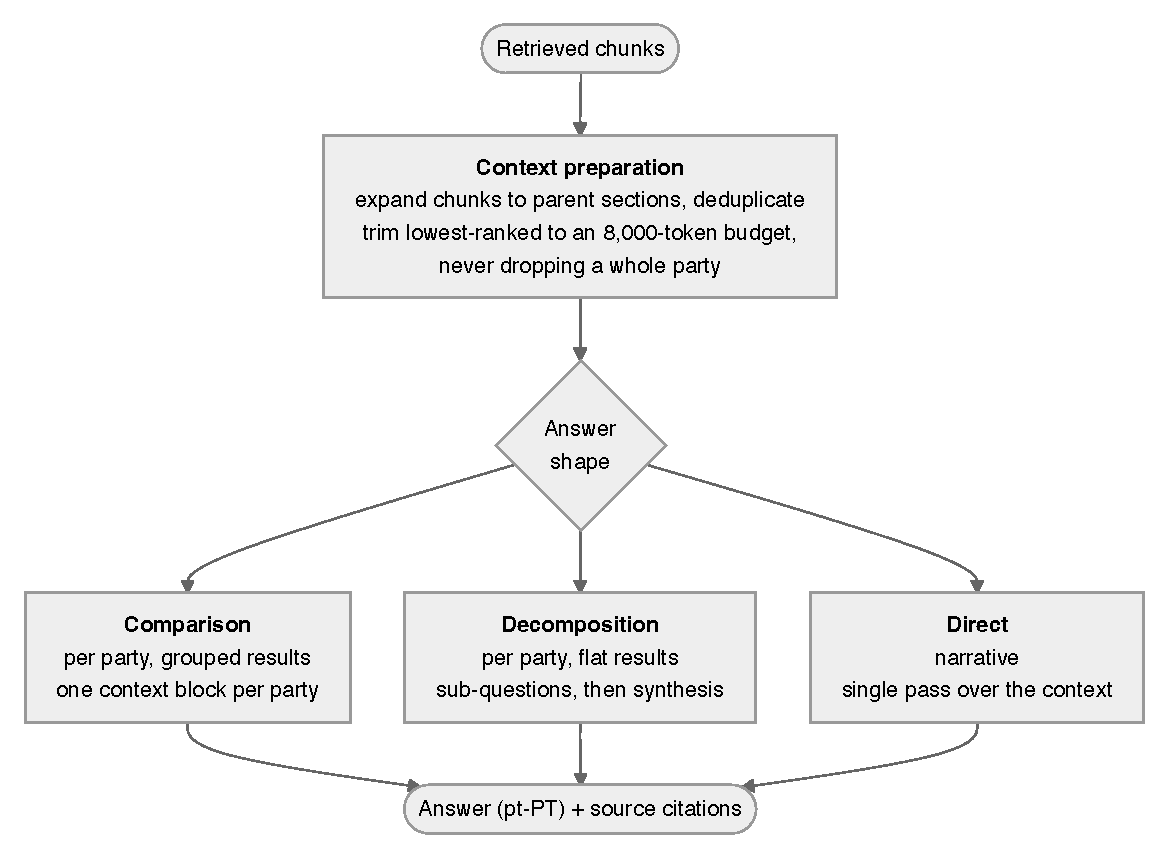
\includegraphics[width=0.9\textwidth]{images/architecture-generation.pdf}
    \caption[Answer synthesis]{Answer synthesis. With no passages to answer from, a fixed reply
    is returned without calling the LLM. Otherwise the context is fitted to the
    prompt budget, and the answer shape set by query analysis picks the
    strategy.}
    \label{fig:generation}
\end{figure}

\subsection{Language model} \label{subsec:llm}

The preliminary research shortlisted four models, two open ones (Llama~3.3
70B and DeepSeek-V3) and two proprietary ones (OpenAI's GPT-4 and Google's
Gemini~2.0 Flash). None of them is used today. Within a year all four had been
overtaken by models that were stronger, cheaper and able to read far longer
inputs, which is one face of the moving-target challenge of
Section~\ref{subsec:challenge-obsolescence}.

%% Source: config/config.yaml (llm.openrouter.model, fallback_models).
Today every LLM role in \sysname{} runs on Google's open-weights Gemma~4. The
26B mixture-of-experts model (\texttt{gemma-4-26b-a4b-it}, with about 4B
parameters active per token) analyses the question, expands it and writes the
answer. The 31B dense model writes the chunk contexts of
Section~\ref{subsec:contextual}. If a call fails, free endpoints are tried in
order, first Gemma~4 31B and then two NVIDIA Nemotron models. The judge comes
from another family on purpose, Qwen (\texttt{qwen3.8-27b}), so no number in
this thesis comes from a model judging its own answers
(Section~\ref{subsec:metrics}). Proprietary models appear only as points of
comparison in the evaluation (Section~\ref{subsec:variants}).

\paragraph{Ways to reach a model.} Gemma on OpenRouter is the fourth and current way
the project reaches a language model. Each of the three before it
was forced by something outside the system, such as cost, hardware or a
provider closing down, rather than by the quality of the answers. The project
started with
small open models run locally through Ollama, at the time the only way to use
an LLM without paying for a subscription or relying on a vendor's free tier.
The laptop at hand could run only small models, though, and their answers
were weak and slow, which slowed down every iteration of the system. Only the
first naive prototype ever ran end to end on a local model. Otherwise local
models served to try out early components, such as an LLM pass that tidied
extracted text.

The second was LlamaAPI, a paid service that routed each call to the model
asked for. A little over a year after it was paid for, it shut down without
notice and took the prepaid credit with it, which made the project wary of
intermediaries for a while. The third was Google's own API, with Gemini~2.5
Flash and Pro. They were inexpensive, came with free credits and wrote good
Portuguese, but the quotas, and having no way to try other vendors' models
through the same interface, eventually became limiting. The fourth, and the
current one, is OpenRouter, which puts many models behind one interface. It
also records which model actually answered each call, so the evaluation
results show whenever a fallback stepped in.

%% Source: commit ec46db9 and the author's note (2026-10-24).
\paragraph{From the free tier to a paid endpoint.} Gemma ran on OpenRouter's
free tier for months, and the free tier shaped the code, with retries and
backoff, fallbacks, and the fail-fast-then-resume design of indexing. It was
evaluation that forced the move to a paid endpoint. One judged run fires
hundreds of calls in a row, and on the free tier a burst like that was
rate-limited almost at once. Each time a rate limit hit, the run had to stop
and wait for it to lift, so a run that takes minutes on the paid endpoint took
hours on the free one. When a limit lasted longer than all the retries put together, the
question was left without a score. The free tier also hands a call to a fallback model when
Gemma is busy, which mixes models inside a single run. The move changed the
bill, not the model. Everything still runs on the same open model, the free
endpoints remain only as a safety net, and no call in the test runs needed
them. On the 36 test questions the production variant spent about \$0.0011 per
answer, and the judge about \$0.0084 more to score it
(Section~\ref{sec:results-cost}).

\subsection{Grounding and neutrality} \label{subsec:grounding}

All prompts are written in European Portuguese, and so are all answers. The
system prompt sets six rules for the answer.
\begin{enumerate}
    \item Answer \emph{only} from the context supplied, never from the model's
    own knowledge.
    \item Cite the source of every claim.
    \item If the context does not contain the answer, reply with one fixed
    sentence, ``Não encontrei resposta a esta pergunta nos excertos dos
    programas que consultei, mas isso não garante que os programas não abordem
    o tema.''\footnote{I found no answer to this question in the manifesto
    excerpts I consulted, but that does not mean the manifestos do not address
    it.}
    \item Describe the measures in neutral language, and attribute every
    justification, diagnosis or value judgement to the party that makes it
    (``o partido considera que\ldots'').\footnote{The party considers
    that\ldots} Never adopt the manifesto's evaluative terms as the system's
    own, and leave out attacks on other parties unless the question asks for
    them.
    \item In comparisons, say explicitly when a party's manifesto does not
    address the topic.
    \item Be direct, with no introduction, no courtesies and no restating of
    the question. Every sentence should carry something concrete from the
    context, such as a measure, a value or a deadline.
\end{enumerate}

The no-answer sentence of rule 3 is worded with care. It says that the
excerpts consulted held no answer, not that the manifestos say nothing on the
subject. The difference matters because retrieval only returns the top $k$
passages, so it can never prove that a manifesto does not mention something.

Refusals are also tracked by the evaluation (Section~\ref{subsec:metrics}). A
judge reads every answer and flags the ones that decline to answer. Some gold
questions cannot be answered from the manifestos, and on those a refusal is the
right outcome, so the evaluation counts how often the system abstains. On the
questions that can be answered, a refusal is a mistake, so it also counts how
often the system refuses wrongly.

Questions about parties outside the corpus get
a different fixed reply (Section~\ref{subsec:queryanalysis}), and the two must
not be confused. One means ``I searched and found nothing'', the other ``I
have nothing to search''.

Query analysis, expansion and generation all run at temperature zero.
Temperature sets how much randomness the model uses when it picks each word,
and at zero it always picks the most likely one, so the same prompt should
produce the same text. This matters for the evaluation. When two variants are
compared, a difference in their scores should come from the setting that
changed between them, not from the model phrasing an answer differently on a
second try. Hosted models do not repeat themselves exactly even at zero, a
limit that Section~\ref{subsec:safeguards} returns to.

\paragraph{Citations.} \label{subsec:citations}
Source transparency is a requirement, not a feature, for a system that
summarises political positions. Every passage in the prompt is numbered,
\texttt{[Documento 1]} to \texttt{[Documento $n$]}, across the whole context,
and carries its party and section path. The model must cite each claim inline
with the matching number, for example \texttt{[2]} or \texttt{[1][3]}. The
answer's list of sources uses the same numbers, so every claim can be traced
to the chunk, section and manifesto it came from, and the evaluation can check
each claim against the passage it cites (Section~\ref{subsec:metrics}). Earlier
prompts asked the model to name the party and section in prose, which named
where information came from, but could not tie a statement to one
specific passage.

\paragraph{Partial answers and false premises.} The first prompts allowed only
two outcomes, a full answer or a refusal. Real questions often fall in
between. The context may cover only part of the question, or the question may
assume something the manifestos do not say. The prompts now ask the model to
answer the part the context supports and to say what the manifestos do not
cover. When a question rests on a premise the context does not confirm, the
model should say so rather than accept it.

%% Source: the framing-leakage TODO and the blind hand count
%% (data/eval/framing/framing-handcount-20261015.json); rule in
%% src/rag/generation/prompts.py (_NEUTRALITY_RULE).
\paragraph{Framing leakage.} Grounding has a side effect. Told to stay close
to the text, the generator repeated each manifesto's framing in the system's
own voice. The answers said that PCP wants to ``romper com a
\emph{submissão} à UE'', that IL wants to repeal ``benefícios fiscais
\emph{dirigistas}'', and that CHEGA wants to make sure immigrants do not
``pretendam \emph{viver de subsídios}''.\footnote{In English, to ``break with
the \emph{submission} to the EU'', ``\emph{state-steered} tax benefits'', and
``intend to \emph{live off benefits}''.} None of this is invented, since every
phrase is in the cited chunk. The problem is whose voice it is in. Each
italicised word is the party's judgement, and the answer states it as plain
fact. This is what \citet{entman1993framing} calls framing, the way a text
presents an issue by choosing what counts as the problem, what caused it and
how it should be judged. The measures themselves came through in neutral
terms. What leaked were the words that carry those judgements. Open attacks
did not survive, and AD's ``caminho socialista'' that ``asfixia'' the
young\footnote{The ``socialist path'' that ``suffocates'' the young.} never
reached an answer. Subtle framing did.

This is not the model's own political lean, which studies measure with no
context at all~\citep{rozado2024political,motoki2024more} and trace to
pretraining data~\citep{pretraining-political-bias}. It is the sources'
framing passing through, and it is uneven. The more rhetorical a manifesto,
the more of its framing gets through.\footnote{Voting advice applications
(Section~\ref{sec:sota-political}) know a version of this problem. The choice
and wording of their statements shape the advice~\citep{walgrave2009statement},
while the tool still looks neutral. In a RAG system the loaded words are not
chosen by the people who built the tool but borrowed from the parties
themselves.}

The comparison prompt already told the model ``Sê imparcial e
factual'',\footnote{Be impartial and factual.} and the leaks above happened
with that line in place. A general request for impartiality does not tell the
model what to do with a party's value words. It was therefore replaced by an
explicit attribution rule, the fourth in the list above, which asks for the
measures in neutral language and for every reason, diagnosis or judgement to be
attributed to the party that makes it. The rule fixed the answers it was
written against.

Whether it did more than that was then checked by hand. All 61 gold questions
were answered once before the rule and once after it. The 122 answers were
shuffled, with nothing to show which run each came from, and every one was
marked against a written rubric. The counts did not move. Both before and after
the rule, 6 of the 61 answers had a clear leak, and 18 had a leak of some kind,
clear or borderline. The leaks themselves did change. Some old ones
disappeared and new ones appeared, mostly in PCP and IL wording.

Two caveats apply. The two runs did not retrieve exactly the same passages,
because query analysis is itself an LLM call, so the comparison is not
perfectly clean. And 61 questions are too few to detect a small effect. The
honest reading is still that the rule made no measurable difference, and that
about one answer in ten repeats a party's framing either way. An instruction
alone is not enough. A check after generation, such as a judge that looks for
unattributed judgements or a pass that rewrites them, is left as future work.
None of the automatic metrics catches the problem
(Section~\ref{subsec:metrics}).

\subsection{Synthesis strategies} \label{subsec:synthesis}

\sysname{} has two ways of writing an answer, called synthesis strategies.
Which one runs depends on the \emph{answer shape}, one of the fields that query
analysis fills in (Section~\ref{subsec:queryanalysis}). It records whether the
user wants one continuous text or an answer laid out party by party.

The \emph{direct} strategy serves the first kind. It puts all the passages
into one prompt, as a single numbered list, and asks for one text. The
\emph{comparison} strategy serves the second. It groups the passages under a
heading for each party, and its prompt asks for each party's position in turn,
followed by a short summary of the similarities and differences. The minimum-wage
question takes this path, as the end of this section shows. The comparison
strategy needs at least two parties with results, and a party-by-party answer
with only one party represented in the answer falls back to the direct strategy.
Before that guard existed, a ``comparison'' of a single party once closed with a
solemn summary that there was nothing to compare.

The strategy follows the answer shape and not the retrieval route, because the
two can differ. ``Que partido propõe mais sobre habitação?''\footnote{Which
party proposes most on housing?} must search every party, so it takes the
comparison route, but it asks for a single verdict rather than eight sections,
so it gets the direct strategy.

\subsection{Fitting the context} \label{subsec:context}

Retrieval returns small chunks, but under small-to-big retrieval the generator
reads each chunk's parent section, or a window of it
(Section~\ref{subsec:chunking}). Several chunks often share a parent, so
passages are deduplicated by the text the generator will read, and overlapping
windows of the same section are merged into one passage. Otherwise one section
could appear two or three times in the same prompt. In one tax question this
took five passages down to three, and about 5,300 tokens down to 2,900.

The context then has to fit a budget of 32,000 tokens. The generation model
runs remotely, so its tokenizer is not available locally, and the budget is
checked with a deliberately cautious estimate of 3.5 characters per token. The
estimate overstates the count, so trimming happens a little early rather than
one passage too late.

When the context is too long, passages have to be dropped, and how they are
dropped depends on the layout. A flat list simply loses its lowest-ranked
passages. A context grouped by party is trimmed one passage at a time, always
from the party that currently has the most, so the parties shrink evenly. No
party is ever trimmed to zero. If one passage per party is already over the
budget, the prompt is sent over the budget anyway. Going over only makes the
prompt longer and leaves a warning in the log, whereas an answer that quietly
leaves out a party looks complete and misleads the reader.

\paragraph{How big a budget.} The budget doubled twice. At 8,000 tokens an
eight-party comparison overflowed with just one passage per party. At 16,000,
when retrieval still sent 24 chunks, the minimum-wage question lost 11 of its
24 passages, 4 of them gold, and scored 0.43 on correctness. At 32,000 nothing
was trimmed and it scored 0.77. One question can justify a setting but not a
headline result, so a budget of 64,000 was then judged against 32,000 on all
61 gold questions. It did no better (correctness 0.014 lower, within noise)
and cost 18\% more input tokens, so the budget stays at 32,000.

\paragraph{No party lost on the way to the answer.} For a question about every
party, the router runs one search per party (Section~\ref{subsec:routing}), so
every party is guaranteed to be \emph{retrieved}. That alone does not
guarantee that every party reaches the \emph{answer}, because the passages
still go through the generator's own steps. Two bugs showed this. Both hit
questions that search every party but ask for a single verdict, such as the
housing question above in synthesis strategy. These use the direct strategy, so the per-party results
have to be turned into one list first.

The first bug was in how that list was built. Besides the per-party results,
the router also returns one overall ranking, cut to the top five passages
(the limit at the time), and the direct strategy read that ranking instead. A
verdict that claimed to weigh eight parties could be written from the passages
of three or four, with nothing in the answer to show it. The direct strategy
now starts from the full per-party results. The second bug was in the trim.
Those results were joined into one list first and trimmed afterwards, so the
lowest-ranked passages went first, and a party whose passages all ranked low
could vanish entirely. They are now trimmed party by party, as described above,
and only then joined into one list.

Two smaller checks catch similar silent failures. If every party's search comes
back empty, the system returns the fixed no-answer sentence directly, instead
of asking the model to answer from an empty context. If the model stops because
it reached the maximum answer length of 3,000 tokens, the answer is marked as
cut off instead of being presented as complete.

%% Source: dev run current-20261015T050000, q-33 (the stored context and
%% answer): 30 passages (AD 5, BE 3, CHEGA 4, IL 3, LIVRE 3, PAN 5, PCP 5,
%% PS 2), 109,152 characters = 31,186 estimated tokens, 26,430 real prompt
%% tokens. The 49 distinct passages come from wide_64k-20261013T051430, the
%% same 64-chunk retrieval at a 64k budget, where nothing was trimmed.
\paragraph{The running example.} Retrieval hands the generator 64 chunks for
the minimum-wage question, eight per party (Section~\ref{subsec:search}). Many
are siblings from the same section, and deduplication merges them into about
49 distinct passages. Those still overflow the budget, so the trim takes
passages from the parties with the most until the estimate falls to about
31,200 tokens. Thirty passages remain, between two and five for every party.
The real prompt, instructions included, came to 26,430 tokens, which shows how
cautious the estimate is.

The analysis asked for a party-by-party answer, so the comparison strategy
builds the prompt. Each party gets a heading, and under it come its numbered
passages, each with its section path. The last passage of the Socialist Party
(PS) opens like this.
\begin{quote}
    \small\ttfamily\raggedright
    [Documento 30]\\
    Secção: PLANO DE AÇÃO PARA PORTUGAL INTEIRO 2024 \textgreater{} \ldots{}
    \textgreater{} 5.1. Trabalho e relações laborais
\end{quote}
Further down, the passage proposes to set, ``em diálogo social na Comissão
Permanente de Concertação Social, uma trajetória plurianual de aumento do
SMN'',\footnote{Through social dialogue in the Standing Committee for Social
Concertation, a multi-year path for raising the national minimum wage.} one
that reaches at least 1,000 euros in 2028. Before that, it notes that the
minimum wage ``cresceu por mais de 60\% desde que o PS é
Governo''.\footnote{Grew by more than 60\% since PS has been in
government.}

The answer has one heading for each of the eight parties and closes with a
short summary. The PS paragraph reads in full as follows.
\begin{quote}
    \small
    \textit{O partido propõe estabelecer, através de diálogo social, uma
    trajetória plurianual de aumento do salário mínimo que permita atingir
    pelo menos 1.000 euros em 2028 [30].}\footnote{The party proposes to
    establish, through social dialogue, a multi-year path for raising the
    minimum wage that reaches at least 1,000 euros in 2028.}
\end{quote}
The citation \texttt{[30]} points to exactly that passage. The claim keeps the
proposal's substance and leaves out the party's praise of its own record,
which is what the neutrality rule asks for. The summary then sets the parties
side by side. PCP wants 1,000 euros already in 2024 and CHEGA by 2026, while
AD, PS and LIVRE set targets for 2028, with LIVRE's 1,150 euros the highest.
IL stands apart by proposing a method for setting the wage rather than a
value. Section~\ref{sec:evaluation} picks the answer up from there and scores
it.

% ============================================================
\section{Evaluation} \label{sec:evaluation}
% ============================================================

Evaluation asks how good each part of \sysname{} is, and how much each
technique adds. Like indexing, it runs ahead of time, against the same vector
store that retrieval searches. Every version of the system it compares runs
the same production code over the same gold questions, and only a few switches
differ between them (Figure~\ref{fig:evaluation}). When two versions differ by
a single switch, the difference in their scores belongs to that one technique.

\begin{figure}[htbp]
    \centering
    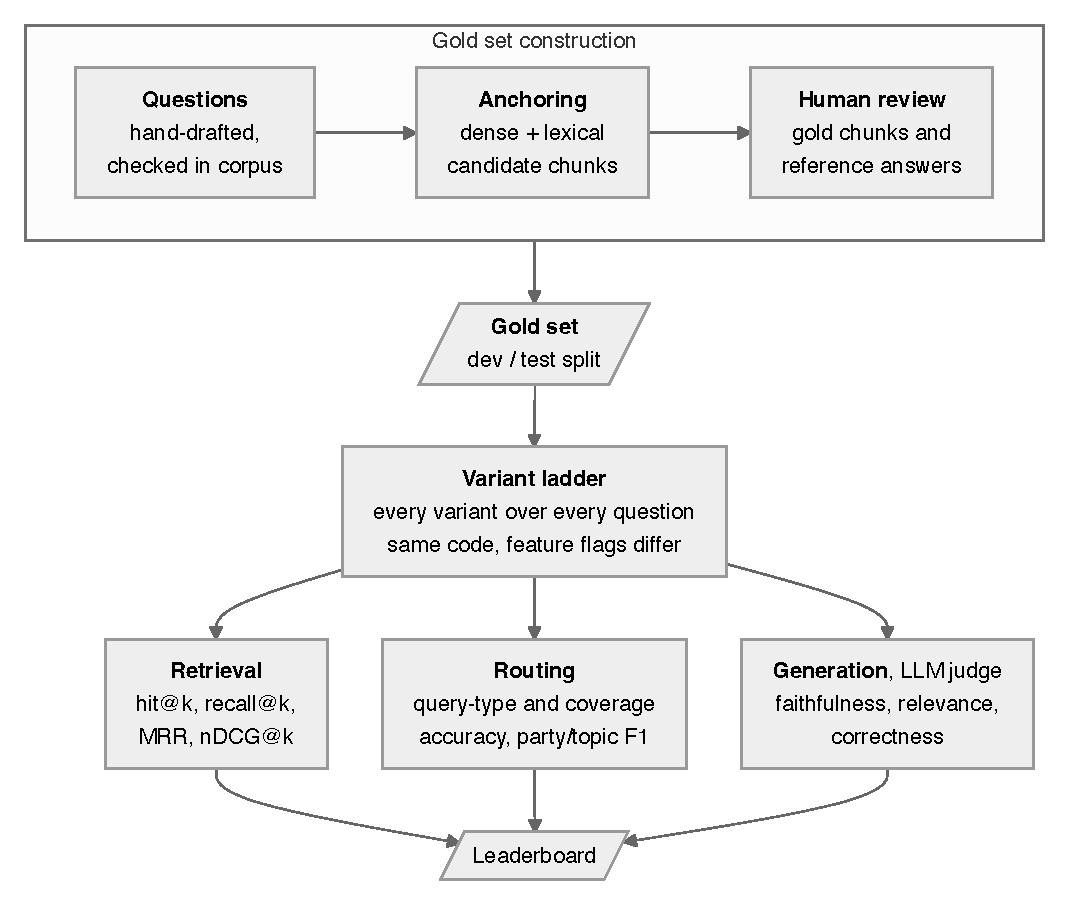
\includegraphics[width=0.85\textwidth]{images/architecture-evaluation.pdf}
    \caption[The evaluation harness]{The evaluation harness. Every variant on
    the ladder runs the same production code over the same gold set. Only the
    feature switches differ.}
    \label{fig:evaluation}
\end{figure}

\subsection{Variant ladder} \label{subsec:variants}
%% Source: docs/evaluation.md §1 and src/rag/evaluation/variants.py.
The original plan was to build three separate RAG systems, a naive one, an
agentic one and one in between, and compare them. It was dropped because two
systems that differ in five ways can be ranked, but nobody can say which of the
five differences made one of them better. \sysname{} has a single pipeline
instead, and every technique beyond plain dense search can be switched on or
off. A \emph{variant} is one combination of these switches. The variants form a
ladder, in which each rung adds one technique to the rung below
(Table~\ref{tab:ladder}), and this ladder is how the step-by-step evaluation
promised in the Introduction is built. Every rung runs the same code over the
same questions, so the difference between two neighbouring rungs is the
contribution of one technique and nothing else. The rungs below
\texttt{current} search an index built without the contextual text of
Section~\ref{subsec:contextual}, so that contextual retrieval also arrives as a
single step.

\begin{table}[htbp]
    \centering
    \small
    \begin{tabular}{|l|p{0.62\textwidth}|}
        \hline
        \textbf{Variant} & \textbf{What it adds} \\
        \hline
        \texttt{naive} & One dense search with the question as typed, and a direct answer \\
        \texttt{multiquery} & Multi-query expansion and RRF fusion \\
        \texttt{routed} & Query analysis and routing, without expansion \\
        \texttt{dense\_only} & Analysis, routing and expansion together \\
        \texttt{hybrid} & BM25 lists fused with the dense ones \\
        \texttt{current} & Contextual retrieval, which gives the production system \\
        \texttt{reranked} & A cross-encoder over 30 candidates \\
        \hline
        \texttt{no\_retrieval} & The production model answering from memory \\
        \texttt{no\_retrieval\_strong} & A frontier model (GPT-5.4) answering from memory \\
        \texttt{current\_strong} & \texttt{current} with the frontier model \\
        \texttt{assistant\_*} & ChatGPT, Gemini and Claude with web search \\
        \hline
    \end{tabular}
    \caption[The variant ladder]{The variant ladder. Above the line, each rung
    adds one technique to the one before. Below it are the points of comparison
    for RQ5. Further variants that each change one setting (the topic filter,
    the prompt budget, an index without the LLM-written context) are listed in
    Appendix~\ref{app:results}.}
    \label{tab:ladder}
\end{table}

The variants below the line answer RQ5, which asks whether \sysname{} beats a
language model answering without retrieval. They switch retrieval off and let
a model answer from what it already knows, with the same rules and the same
maximum answer length. \texttt{no\_retrieval} is the production model
answering from memory, and \texttt{no\_retrieval\_strong} does the same with
GPT-5.4, a much larger model from a third family. \texttt{current\_strong}
gives that larger model the production retrieval. The \texttt{assistant\_*}
rungs are what a citizen gets today by asking a commercial chatbot, ChatGPT,
Gemini or Claude with web search on, free to find the manifestos for itself.
Without retrieval there is no context to check an answer against, so these
rungs are scored only on correctness, relevance, abstention and cost.

\subsection{Gold set construction} \label{subsec:goldset}
%% Source: docs/evaluation.md §2, data/eval/questions/CANDIDATES.md,
%% scripts/anchor_gold.py, anchoring/ANCHORING.md and golden.json.
No question-answering dataset exists for Portuguese manifestos, so one was
built for this work. It has 61 questions. Each one carries the passages of the
manifestos that answer it, called its \emph{gold chunks}, and a reference
answer. The minimum-wage question, for instance, has 20 gold chunks from 17
sections of the eight manifestos, and a reference answer that gives each
party's target in a sentence or two.

The set was built in four steps. First, the questions were written by hand.
Fifty-one were written against the eight manifestos, each with a note on where
its answer lies, checked against the indexed text. The note also records the
route the question should take (its parties, topics and coverage), the rung of
the ladder it is meant to test, and how hard it is expected to be. Ten probes
were then added to test behaviour rather than recall. Seven cannot be answered
from the manifestos and test whether the system declines, among them q-59 on a
party outside the corpus. Two can be answered only in part, and q-61 asks about
a single passing mention.

Second, a script gathered candidate chunks for each question and each party it
names, by dense search and by short keyword searches. Third, an LLM (Claude)
proposed the gold chunks and a reference answer for each question, from those
candidates and the note. Every proposal was then reviewed by hand. Picks were
fixed, references rewritten and each question marked as reviewed, and all 61
went through this review. The proposals are kept, so every change made in
review can be seen. Last, the reviewed set is compiled into one file. Each
question's route is derived from its parties and coverage by the same rule the
pipeline uses (Section~\ref{subsec:queryanalysis}), so the routing metrics get
their expected answers without any extra labelling.

Some questions are broad on purpose. q-42 asks ``Que apoios são propostos
para pessoas com deficiência?''\footnote{What support is proposed for people
with disabilities?} and has 88 gold chunks from 58 sections. Narrowing such a
question to suit the system would hide exactly the kind of question users ask.
The gold for a broad question is every chunk in the section a party gives to
the topic, plus explicit proposals on it found elsewhere. Pure diagnosis, past
achievements and budget tables are left out.

Gold chunks are identified by a hash of their text rather than by a database
id, so the gold set survives a re-index as long as the chunks themselves do not
change. The questions are split into 25 for development and 36 for testing,
balanced across route, party and difficulty. Over the whole set there are 26
single-party questions, 20 comparisons, 10 topic explorations and 5 general
ones.

%% Reasons for dropping the synthetic plan confirmed by the author (2026-10-24).
The questions were not always meant to be written by hand. The first plan was
to sample chunks and have an LLM write a question for each, with the sampled
chunk as its gold. It was dropped for two reasons. A question written from a
chunk borrows that chunk's words, so dense and lexical search find it far more
easily than they would find a real user's question. And a test written by an
LLM would grade LLMs on questions shaped by an LLM, the kind of circularity the
separate judge family is there to avoid (Section~\ref{subsec:metrics}). The LLM
proposals of the third step carry a milder form of the same risk, which is why
every one of them was reviewed by hand.

%% Keep every sentence true: three revisions were judged on all 61 questions
%% (commits 524d9ea and b054bf8) and q-59 (a test question) motivated the
%% out-of-corpus revision, so do NOT claim tuning used dev questions only or
%% that test was never seen. Numbers: data/eval/extras/dev-only-recheck.md
%% (scripts/eval_extras/dev_only_recheck.py).
\paragraph{Which questions shaped the system.} The system was built while the
gold set was still being written, and each revision in this chapter says which
questions it was measured on. The split into development and test questions
was fixed when the gold set was finished, and most revisions were chosen on the
25 development questions alone. Three late ones were judged on all 61 questions
instead, to make their intervals narrower. These were contextual retrieval
(Section~\ref{subsec:contextual}), retrieving more chunks without the topic
filter (Section~\ref{subsec:routing}) and the larger prompt budget
(Section~\ref{subsec:context}). Re-checked on the development questions alone,
all three point the same way. Retrieving more chunks keeps a clear gain (recall
+0.141, with a 95\% confidence interval from +0.08 to +0.22), and the larger
budget still reads no better. Contextual retrieval keeps its direction, but
with intervals that include zero (recall +0.034, nDCG +0.032), so its gain on
the test questions is not fully independent of the decision to adopt it. One
bug fix also came from a test question. The answer to q-59 showed that a party
outside the corpus could be mistaken for one inside it
(Section~\ref{subsec:queryanalysis}). The numbers in Chapter~\ref{ch:results}
come from a single run of every variant on the 36 test questions, on code that
was frozen before that run and not changed afterwards. That code is commit
\texttt{0293a0b}, tagged \texttt{code-freeze}, and every result records it as
its \texttt{code\_version}.

\paragraph{Neutral references.} The reference answers follow a written rule,
much like the one later given to the generator
(Section~\ref{subsec:grounding}). They describe each measure in neutral
language, and they give a party's reasons only as the party's own claims, with
phrases such as ``argumenta que'' or ``por considerar que''.\footnote{``Argues
that'' and ``because it considers that''.} They never adopt a party's
evaluative terms, and they leave out attacks on other parties. The rule was
added during the review, after five references already marked as reviewed
turned out to carry the parties' framing. The reference for q-08 spoke of PCP's
``submissão'' to the EU, and the one for q-18 of IL's ``desperdício'' of
votes.\footnote{``Submission'' and ``waste''.} Framing like this is easy to
miss while reading, so it needs a written rule rather than good intentions. A
correct reference reads like q-04, where bullfighting is something PAN
``considera um erro civilizacional'', or q-47, which opens ``Segundo o programa
do CHEGA''.\footnote{``Considers a civilisational error'' and ``according to
the CHEGA manifesto''.}

\subsection{Metrics} \label{subsec:metrics}
%% Source: docs/evaluation.md §3 and src/rag/evaluation/metrics/.
Three families of metrics score each run, one for each stage of the pipeline.

\paragraph{Retrieval.} Retrieval is scored against the gold chunks with the
standard metrics of information retrieval (Section~\ref{subsec:sota-metrics}),
computed over the full list of chunks handed to generation. \emph{Hit rate}
asks whether at least one gold chunk was found, and \emph{recall} what share of
them was found. \emph{MRR} looks at how high the first gold chunk ranks, and
\emph{nDCG} at how high all of them rank. Broad questions need two more. A
question can have more gold chunks than the system retrieves. q-42 has 88,
while the system retrieves at most 64, so \emph{capped recall} divides by
whichever of the two is smaller. \emph{Aspect recall} counts manifesto sections
instead of chunks, since ten chunks from one section cover less of a broad
answer than three chunks from three different sections. Unlike the context
metrics of RAGAs, none of these needs a judge. They are exact, cost nothing,
and two of them take the order of the list into account.

\paragraph{Routing.} Query analysis is scored against the route each question
is expected to take. The scores are the accuracy of the derived query type, F1
over the parties and the topics it extracts, and \emph{coverage accuracy}. The
last one catches the costliest mistake, a question about every party answered
from a single search that leaves half of them out.

\paragraph{Generation.} Answers are scored claim by claim, following
RAGAs~\citep{es2024ragas}. The judge first breaks an answer into short claims
that each state one fact. \emph{Faithfulness} is the share of those claims
supported by the context the generator read. \emph{Correctness} compares the
answer's claims with the claims of the reference answer. Its precision is the
share of the answer's claims found in the reference, its recall the share of
the reference's claims found in the answer, and correctness is the F1 of the
two. Recall on its own, called \emph{correctness recall}, says how much of the
reference an answer covers. Last, a \emph{relevance} judgement scores from 1 to
5 whether the answer addresses the question. It also records whether the
answer declined to answer, which gives two more measures. \emph{Abstention} is
the share of unanswerable questions the system declined, and \emph{false
refusal} the share of answerable ones it wrongly declined.

%% Source: dev run current-20261015T050000, q-33 (metrics and judgements):
%% recall 0.90, MRR 1.0, aspect recall 15/17, faithfulness 27/27,
%% correctness recall 14/16, precision 18/27, correctness 0.757.
\paragraph{The running example.} In a development run, retrieval found 18 of
the 20 gold chunks for the minimum-wage question (recall 0.90), with a gold
chunk in first place (MRR 1.0), and the chunks it found come from 15 of the 17
gold sections (aspect recall 0.88). Query analysis got every part of the route
right. All 27 claims of the answer are supported by the passages it read, so
faithfulness is 1.0. Correctness tells a different story. The answer covers 14
of the 16 claims of the reference, a correctness recall of 0.88, and misses,
for instance, PAN's call for a more ambitious European minimum wage. But only
18 of its 27 claims appear in the reference, which pulls correctness down to
0.76. The other nine come straight from the passages, such as IL's plan to
transpose the European directive on minimum wages. The reference, at a
sentence or two per party, simply leaves them out. Correctness precision
punishes detail that the reference did not include, which is why
Chapter~\ref{ch:results} reports correctness recall alongside correctness.

\paragraph{The judge.} Every generation metric is computed by an LLM judge,
and LLM judges tend to favour answers written by their own model
family~\citep{zheng2023judging}. The judge is therefore Qwen
(\texttt{qwen3.8-27b}), a family different from both the Gemma generator and
the GPT model of the RQ5 comparisons. A judge call that fails leaves its score
out rather than recording a zero.

%% Source: data/eval/extras/judge-validation.md (full figures, PABAK and the
%% confusion counts).
\paragraph{Checking the judge.} A judge is only useful if it agrees with a
careful reader, so its verdicts were compared with ratings made by hand. The
sample was 25 production answers from the test questions, 1,088 claims in
all, and each claim was rated without seeing the judge's verdict. Correctness
recall holds up well. The two agree on 95\% of claims, with a Cohen's $\kappa$
of 0.90 (a measure of agreement that discounts what chance alone would give),
and where they disagree the judge is usually the stricter.

Faithfulness agrees on 98.9\% of claims, but that figure proves little. Nearly
every claim of the production system is supported, so a judge that accepted
everything would score almost as well. To test whether the judge can reject a
claim, twelve closed-book answers were judged against the passages that the
production variant had retrieved for the same questions. Those answers were
written without the passages, so about two in five of their claims are not
supported by them. The judge caught 89\% of the claims rejected by hand. Most
of its extra rejections were strict readings of an embellishment whose
substance the passages did support, such as calling something the
``principal motor''\footnote{Main driver.} of a policy. Its blind spot is
absence. It credited a refusal with the reference claim that ``nenhum outro
programa indica'' the year,\footnote{No other manifesto gives (the year).}
and it passed ``os programas não indicam o ano''\footnote{The manifestos do
not give the year.} while its own reasoning cited the manifesto that does.

Relevance is the weakest of the three. The judge gave the top mark to 22 of
the 25 production answers, and also to 10 of 12 closed-book answers that got
almost nothing right. Relevance therefore says whether an answer is on topic,
not whether it is correct. It is never used to rank variants, and it is read
only through its record of whether the answer declined, for abstention and
false refusal.

\paragraph{Faithfulness is not neutrality.} Faithfulness asks whether the
sources say a claim. It never asks whether the claim is true, or whose view it
is. To show this, the judge was given three claims against the context of q-08.
The first was that PCP ``defende romper com a submissão à União Europeia'', the
second the same claim with the word attributed to the party (``aquilo a que o
partido chama submissão''), and the third ``Portugal está numa situação de
submissão à União Europeia'', with no party named at all.\footnote{In English,
PCP ``advocates breaking with submission to the European Union'', ``what the
party calls submission'' and ``Portugal is in a situation of submission to the
European Union''.} It accepted all three. Faithfulness assumes that the context
is a trustworthy reference. In a corpus of manifestos, which are partisan by
design, that assumption fails. A claim can be faithful to its source and still
adopt the source's framing, and the metric cannot tell the difference. This is
not a flaw of this implementation, which follows the RAGAs recipe step by step,
nor something RAGAs claims to cover. The metric was never meant to measure
neutrality, and the RAGAs paper validates it on Wikipedia pages. Correctness
has the same blind spot whenever the reference carries the same framing, which
is why the references follow an attribution rule
(Section~\ref{subsec:goldset}). Framing leakage is therefore counted by hand
(Section~\ref{subsec:grounding}).

\paragraph{No layer is neutral.} Every safeguard in this evaluation is a check
made by someone, or something, with views of its own. The generator and the
judge are language models, and chat models show political leanings of their
own, most of them left of centre~\citep{rozado2024political,motoki2024more}. A
judge from another family guards against a model favouring its own kind, but
it brings a different leaning, and a different leaning is still not none. The
prompts that tell both models to stay neutral were written by a person. So
were the questions, the gold chunks and their references, the count of framing
leaks and the ratings that check the judge. All of these were made by the same
person who built the system, and nobody is free of political views. Those
views are not disclosed here, since the system is meant to be judged without
them. They still exist, and they can shape the small calls these checks are
made of, such as whether a phrase reads as a party's framing or as plain
description, or whether an answer covers a reference well enough. Each layer
therefore narrows the room for bias without closing it. The ratings that check
the judge were made without its verdicts in view, and the references keep
every value-laden statement in the voice of its party
(Section~\ref{subsec:goldset}). A check by hand is still a second opinion
rather than the truth. The proper remedy, several raters from across the
political spectrum and a measure of how far they agree, was beyond the means
of this work (Chapter~\ref{ch:conclusion}).

\subsection{Measurement safeguards} \label{subsec:safeguards}
%% Source: evaluation/models.py (label validator), runner.py (strict mode),
%% metrics/generation.py (omitted scores), reranker.py, report.py (models_used),
%% retrieval/query_analyzer.py (_ANALYSES, commit 71cf9d7),
%% tests/integration/test_filtered_vector_search.py,
%% tests/unit/indexing/test_contextual_embedding.py.
A comparison between variants is only as good as the numbers on both sides.
Several failures in this pipeline would raise no error and would instead
quietly change a score. Each of the ones below is therefore checked
automatically, either by the evaluation harness or by a test in the
repository's test suite.

\paragraph{Gold labels that agree.} Each gold question's route is derived from
its parties and coverage, exactly as the pipeline derives it. A question whose
labels contradict each other is rejected when the gold set is loaded, instead
of quietly scoring zero on every variant.

\paragraph{Failures are errors, not scores.} When query analysis or expansion
still fails after its retries, the system normally falls back to a simpler
pipeline, so that the user still gets an answer
(Section~\ref{subsec:queryanalysis}). In an evaluation, that answer would be
scored under the variant's name while coming from a different pipeline. The
harness therefore runs both steps in a strict mode, in which such a failure is
recorded as an error for that question. In the same way, a judge call that
fails leaves its score out instead of recording a zero, so an outage at the
provider cannot pass for a bad answer.

\paragraph{Filtered searches that return everything.} pgvector applies
metadata filters after its approximate index scan (HNSW), so a filtered query
can return fewer rows than it asked for. Measured here, a party filter under an
HNSW plan returned 3 of the 30 rows requested, as the pgvector documentation
warns~\citep{pgvector}. At the current corpus size, PostgreSQL plans a
party-filtered search with an ordinary index on the party column and an exact
sort instead, so the results are complete. A test on a table shaped like the
real one, with the same number of chunks per party and the same vector size,
checks that a party-filtered search returns the full top-$k$. If the corpus
grows or a pgvector upgrade switches the plan to HNSW, the test fails instead
of retrieval silently receiving fewer passages.

\paragraph{One gold set for every index.} Gold chunks are identified by a hash
of their text (Section~\ref{subsec:goldset}). Contextual retrieval adds
headers and an LLM-written context to the text that is embedded, so a test
checks that it changes only that text and never the stored content of a chunk.
The same gold set can then score every variant, whichever index it searches.

\paragraph{No silent substitutions.} A reranker that fails to load stops the
run, instead of returning results that were never reranked under the
\texttt{reranked} name. An answer cut off at the maximum length is marked in
its record, and the leaderboard notes any variant in which a fallback model
answered some of the calls.

\paragraph{Noise without repeated runs.} Hosted models do not repeat
themselves exactly, even at temperature zero. Two identical runs over the 61
questions retrieved the same chunks for only 10 of them, and recall moved by up
to 0.03, which is as large as some of the effects being measured. Repeating
every run several times would multiply a cost already counted in dollars, so
two other safeguards stand in for repetition. First, within one evaluation run
every variant reuses each question's query analysis and reformulations, which
are computed only once. The variants then differ only in the technique under
test, and this is why the headline ladder runs in a single invocation. Second,
every difference between two variants is reported with a 95\% confidence
interval from a paired bootstrap. The bootstrap resamples the questions many
times and recomputes the difference each time, and the interval holds the
middle 95\% of those differences. A difference whose interval includes zero
could be noise, and it is not read as a result.

% ============================================================
\section{What building it taught} \label{sec:lessons}
% ============================================================
%% DRAFT (Claude, 2026-10-25): closing lessons. Rewrite in your own words.
The multiple revisions in this chapter were not random. Read together, they come down
to four lessons, each paid for by at least one failure.

\paragraph{Quiet failures are the worst.} Several failures in this chapter
produced answers that looked fine. The encoder read only the first 128 tokens
of each chunk, so about two thirds of the corpus was never embedded
(Section~\ref{subsec:chunking}). Lexical search demanded every word of the
question, so hybrid retrieval ran as dense search alone
(Section~\ref{subsec:search}). A keyword fallback mixed crude labels with LLM
labels (Section~\ref{subsec:classification}), a topic filter emptied the search
(Section~\ref{subsec:routing}), ``PSD'' matched the Partido Socialista, and ADN
was answered as AD (Section~\ref{subsec:queryanalysis}). None of them raised an
error, and most came with tidy citations. Two habits came out of them. Every
limit is measured in the unit that sets it, which for an encoder means tokens
rather than characters. And a step that cannot do its job stops or says so,
instead of quietly doing something smaller (Section~\ref{subsec:safeguards}).

\paragraph{Each step must be fair.} Searching each party
separately guarantees that every party is retrieved
(Section~\ref{subsec:routing}). It does not guarantee that every party reaches
the answer. A narrative verdict was once written from the top five passages of
an eight-party search, and a grouped context was once trimmed as a flat list,
which could drop a low-ranking party altogether
(Section~\ref{subsec:context}). Both defects sat after the step that was meant
to make the system fair. Fairness is a property of the whole path from
question to answer, and every step that cuts, trims or ranks has to be checked
for the party it might leave behind.

\paragraph{One cannot just tell the model to be neutral.} Telling the model to be
impartial did not help, and the more precise attribution rule that replaced
it had no measurable effect. About one answer in ten still repeats a party's
framing (Section~\ref{subsec:grounding}). The metrics do not see it either. A
judge checking faithfulness accepts a party's framing as long as the source
says it (Section~\ref{subsec:metrics}), and the reference answers carried the
same framing until a written rule removed it (Section~\ref{subsec:goldset}).
What helps is making political choices explicit and checkable, such as
resolving ``the right-wing parties'' through a published scale rather than the
model's own view (Section~\ref{subsec:queryanalysis}), and admitting that every
check, the author's included, comes from someone with views.

\paragraph{Measure first, believe later.} Several techniques that looked like
clear improvements did not survive measurement. The cross-encoder reranker cut
recall (Section~\ref{subsec:reranking}), the
topic filter excluded the passages it was meant to find
(Section~\ref{subsec:routing}), and doubling the prompt budget read no better
(Section~\ref{subsec:context}). Contextual retrieval and BM25, both simple,
earned their place. None of this would have been visible without the switches
that let each technique be turned off and measured on its own
(Section~\ref{subsec:variants}).

Together, these make \sysname{} less a pipeline of techniques than a set of
guarantees, each one bought with a failure. What it already does is modest and
useful. A citizen can ask any question about the 2024 manifestos, in European
Portuguese, and get an answer that covers every party in scope and points to
the passage behind each claim, for a fraction of a cent. A version with more
resources could cover every party on the ballot and every election, and follow
how positions change from one manifesto to the next
(Chapter~\ref{ch:conclusion}). Whether its answers are right often enough to be
trusted is a question for measurement, and Chapter~\ref{ch:results} takes it
up.
